%\documentclass[a4paper,]{book}
\documentclass[a4paper, twoside,openright ,titlepage, 12pt]{book}
\usepackage[english]{babel}
\usepackage{preamble}

\usepackage[MEK, 60]{masterfrontpage}
\title{A comparison of }
\subtitle{Valgfri underoverskrift}
\author{Andreas Slyngstad}
%\setlength\parindent{0pt}

\begin{document}                                                                                                                          
%\maketitle
\masterfrontpage
\section*{Acknowledgements}
First off, I would like to my supervisors Dr. Kristian Valen-Sendstad and Aslak Wigdahl Bergersen. Kristian, your encouragement .. Aslak, numerical insight and problem solving methodology have been mostly a

I would also like to thank Professor Mikael Mortensen and Miroslav Kuchta at the Department of Mathematics at the University of Oslo. Your technical insight in the FEniCS project have been essential for completing this thesis. 

Finally I would like to thank my partner Charlotte and daughter Linde Olivia. Your love and support have kept me motivated during this thesis, would not and for giving me something to look

\pagenumbering{roman}
\tableofcontents
\newtheorem{theorem}{Theorem}[section]
\newtheorem{lemma}[theorem]{Lemma}
\pagenumbering{arabic}

\chapter{A motivation for studying fluid-structure interaction}
The interaction between fluid and solids can be observed all around us in nature and has shown crucial in engineering. Examples in nature include swimming fish, flying birds, or trees bending in the wind. Man has learned from nature and has traditionally relied upon laboratory experiments to design windmills, aircrafts, and bridges. The importance of understanding fluid-structure (or solids) interaction (FSI) cannot be overstated, as the lack of such has demonstrated to be disastrous in the design of everything from bridges to airplanes. Let alone to emphasize our incapability to replicate the performance of nature; we're far away from designing a drone capable of flying like a hummingbird. However, laboratory experiments are inherently noisy, expensive, and results can be difficult to reproduce. A much cheaper and indeed smarter approach to studying FSI is using computers, or more specifically numerical simulations to gain fundamental insight to the interaction between fluids and solids. The latter has on the other hand shown to be difficult to realize, for a number of reasons related to both mathematical and computational reasons. Therefore, the goal of this thesis is to develop an open-source framework using standard techniques for solving FSI problems that can be used as a point of reference for future benchmarking of FEniCS-based FSI solvers. \\

The main goal of this thesis is to create a verified and validated monolithic fluid-structure interaction solver in FEniCS, which can handle large deformations. To achieve this, I have defined four subgoals: 

\begin{itemize}
\item Formulate a weak variation for a monolithic arbitrary Lagrangian Eulerian fluid-structure interaction problem.
\item Construct a finite element solver for the fluid-structure interaction problem.
\item Verify and validate a finite element solver for the fluid-structure interaction problem.
\item Compare the impact of discretization and mesh lifting operators on the final solution.
\item Improve computational efficiency of the implementation.
\end{itemize}


Each of the following subgoals will be addressed in separate chapters organized as follows: Balance of linear momentum for both solids and fluids are first introduced together with conservation of mass. The Eulerian, Lagrangian, and the arbitrary Lagrangian-Eulerian (ALE) frames of reference are briefly introduced to express the governing equations, before the equations describing FSI are derived. The numerical implementation is verified using the most rigorous convergence tests, before validation is performed against state-of-the-art benchmarks. Finally, computational speed-up is addressed together with long-term numerical stability of the coupled problem, and methods to overcome these challenges.
 

\chapter{Governing equations}

Computational fluid-structure interaction (CFSI) combines two separate fields of computational mechanics, computational fluid dynamics (CFD), and computational structure dynamics (CSM). While CFD and CSM traditionally have been considered as two distinct fields of science,  the goal of CFSI is to combine the separate fluid and structure problems ,and their interaction or \textit{coupling} to one another. Therefore, the study CFSI demands understanding of each separate field. This chapter presents the governing equations of the individual fluid and structure problem. Balance laws for each separate problem,  together with auxiliary kinematic, dynamic and material relations will be described briefly.


\section{Continuum Mechanics}
In our effort to understand and describe physical phenomenon in nature, we describe our observations and theories by creating mathematical models. The mathematical models makes scientist and engineers not only able to understand physical phenomena, but also predict them.  All matter is built up by a sequence of atoms, meaning on a microscopic level, an observer will locate discontinuties and space within the material. Evaluating each atom, or \textit{material point}, is not impossible from a mathematical point of view. However, for mathematical moddeling and applications, the evaluation of each material point remains unpractical. In \textit{continuum mechanics}, first formulated by Augustin-Louis Cauchy \cite{Merodio2011}, the microscopic structure of materials are ignored,  assuming the material of interest is \textit{continuously distributed} in space, referred to as a continuum.


In context of this thesis we define a \textit{continuum} as a continuous body $V(t) \subset \mathbb{R}^d \ d \in (1, 2, 3)$ ,  continuously distributed throughout its own extension. The continuum is assumed to be infinitely divisible, meaning one can divide some region of the continuum a indefinitely number of times. A continuum is also assumed to be locally homogeneous, meaning if a continuum is subdivided into infinitesimal regions, they would all have the same properties such as mass density. These two properties forms the baseline for deriving conservation laws and constitute equations, which are essential for formulating mathematical models for the material of interest. However, a continuum remains a mathematical idealization, and may not be a reasonable model for certain applications. In general, continuum mechanics have proven to be applicable provided that $\frac{\delta}{l} << 1$ where $\delta$ is a characteristic length scale of the material micro-structure, and $l$ is a length scale of the problem of interest \cite{Humphrey2002}.

\section{The Lagrangian and Eulerian description of motion}
In continuum mechanics, one makes use if two classical description of motion, the \textit{Lagrangian} and \textit{Eulerian} description. Both concepts are related to an observers view of motion, visually explained by the concepts of \textit{material} and \textit{spatial} points. A material points represents a particle within the material, moving with the material as it move and deform. A spatial point, refers to some reference at which the path of the material points are measured from. 

\begin{figure}[h!]
  \centering
    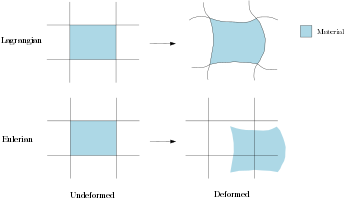
\includegraphics[scale=0.9]{./Fig/lageul.png}
      \caption{Comparison of the Lagrangian and Eulerian description of motion}
\end{figure}


\subsubsection*{Lagrangian}
In the Lagrangian description of motion, the material and spatial points coincide, meaning the reference point of which motion is measured, follows the material as it diverts from its initial position. The initial position of all material points in a continuum extend a region, called the \textit{reference configuration} $\hat{V}$. From now on, all identities in the \textit{reference configuration} will be denoted with the notation "$\wedge$". If a continuum deviates from its reference configuration, a material point $\bat{x}(x, y, z ,t)$ may no longer be at its initial position, but moved to a new position $\mathbf{x}(x, y, z, t)$ at time $t$.  The new positions of all material points extend a new region, called the \textit{current configuration} $V(t)$. 
\newpage

\begin{figure}[h!]
  \centering
    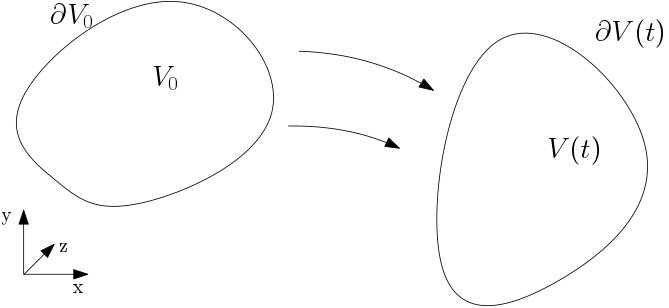
\includegraphics[scale=0.4]{./Fig/unitpotato.png}
      \caption{Unitpotato}
\end{figure}

To measure the displacement of a material point $\mathbf{x} \in V(t)$ for time $t$, from its initial point $\bat{x} \in \hat{V}$, one defines a \textit{deformation vector field} 

\begin{align}
\bat{u}(\ha{x},t) = x(\bat{x},t) - \bat{x} = \ha{T}(\bat{x}, t) 
\end{align}

Mathematically, deformation is a 1:1 mapping  $\ha{T}(\bat{x}, t)$, transforming material points from the   \textit{reference configuration} $\hat{V}$, to the  \textit{current configuration} $V(t)$. Visually, the deformation resembles the shape of continuum for some time $t$. To describe the continuums motion, one defines the \textit{velocity vector field} given by the time derivative of the deformation field,
\begin{align}
\bat{v}(\ha{x},t) = d_t x(\bat{x},t) = d_t \bat{u}(\bat{x},t) = \pder{\ha{T}(\ha{x}, t)}{t} 
\end{align}

The Lagrangian description of motion is the natural choice when tracking particles and surfaces are of main interest. Therefore, it is mainly used within structure mechanics. 

%http://www.brown.edu/Departments/Engineering/Courses/En221/Notes/Kinematics/Kinematics.htm
%Arbitrary Lagrangian-Eulerian methods J. Donea1
\subsubsection*{Eulerian}
 In the Eulerian description, the reference point is kept fixed while the material is deformed.

%The initial shape of the continuum, the \textit{reference configuration}  $V(t = t_0) = \hat{V}$,  is assumed to be stress free.   When the \textit{continuum} undergoes deformation due to applied internal or external forces , the new configuration $V(t)$ for $t \geq t_0$, deviates from its \textit{reference configuration}. The new configuration  $V(t) \neq \hat{V}$, is defined as the \textit{current configuration}. If the continuum undergoes no deformation, the  \textit{reference} and \textit{current} configuration simply coincide. \\ \\




Considering a flow of fluid particles in a river, a \textit{Lagrangian} description of the particles would be tedious as the number of particles entering and leaving the domain quickly rise to a immense number. 
Instead consider defining a view-point $V$ fixed in time, and monitor every fluid particle passing the coordinate $x \in V(t)$ as time elapses. Such a description is defined as the \textit{Eulerian framework.} 
Therefore the Eulerian formulation is natural for describing fluid dynamics. \\
We can describe the particles occupying the \textit{current configuration} $V(t)$ for some time $t \geq t_0$ 
\begin{align*}
x = \ha{x} + \hat{u}(\ha{x}, t)	
\end{align*}
Since our domain is fixed we can define the deformation for a particle 
occupying position $x = x(\ha{x},t)$ as
\begin{align*}
\textbf{u}(x, t) = \hat{u}(\ha{x}, t) = x - \ha{x}	\\
\end{align*}
and its velocity
\begin{align*}
\textbf{v}(x,t) = \partial_t u(x,t) = \partial_t \hat{u}(\ha{x},t) = \hat{v}(\ha{x},t)
\end{align*}

It is important to mention that the we are not interested in which particle is occupying a certain point in our domain, but only its properties. 
%When tracking each particle as it moves, the \textit{material} and \textit{spatial} %points coincide
%As such the \textit{material} and \textit{spatial} points doesn't coincide in the %\textit{Eulerian formulation}

\section{The deformation gradient}
Deformation is a major property of interest when a continuum is influenced by external and internal forces.  The deformation results in relative change of position of material particles, called \textit{strain}. and is the primary property that causes and describe \textit{stress}.

Strain is purely an observation, and it is not dependent on the material of interest. However one expects that a material undergoing strain, will give  forces within a continuum due to neighboring material particles interacting with one another. Therefore one derive material specific models to describe how a certain material will react to a certain amount of strain.
These strain measures are used to define models for \textit{stress}, which is responsible for the deformation in materials \cite{Holzapfel2000}. Stress is defined as the internal forces that particles within a continuous material exert on each other, with dimension force per unit area.  \\

The equations of continuum mechanics can be derived with respect to either a deformed or undeformend configuration. The choice of refering our equations to the current or reference configuration is indifferent from a theoretical point of view. In practice however this choice can have a severe impact on our strategy of solution methods and physical of modelling.   \cite{Wriggers2006}. Regardless of configuration, the \textit{deformation gradient} and \textit{determinant of the deformation gradient} are essential measurement in structure mechanics. 
By \cite{Richter2016}, both configurations are considered.


\subsubsection*{Reference configuration}
\begin{defn}
Let $\hat{u}$ be a differential deformation field in the \textit{reference} configuration, $I$ be the Identity matrix and
the gradient $\hat{\nabla} = (\frac{\partial}{\partial x}, \frac{\partial}{\partial y}, \frac{\partial}{\partial z}) $. Then the \textit{deformation gradient} is given by,
\begin{align}
\bat{F} = I + \hat{\nabla} \bat{u} 
\end{align} 
\textit{expressing the local change of relative position under deformation.}
\end{defn}

\begin{defn}
Let $\hat{u}$ be a differential deformation field in the \textit{reference} configuration, $I$ be the Identity matrix and
the gradient $\hat{\nabla} = (\frac{\partial}{\partial x}, \frac{\partial}{\partial y}, \frac{\partial}{\partial z}) $. Then the \textit{determinant of the deformation gradient} is given by,
\begin{align}
J = det(\bat{F}) = det( I + \hat{\nabla} \bat{u} )
\end{align} 
\textit{expressing the local change of volume the configuration.}
\end{defn}

From the assumption of linear operator \textbf{F}, and no two particles $\bat{x}_a, \bat{x}_b \in \ha{V}$ occupy the same location for some time $V(t)$,  J to be greater than 0 \cite{Wriggers2006}. \\ \\

\subsubsection*{Current configuration}
\begin{defn}
Let $\mathbf{u}$ be a differential deformation field in the \textit{reference} configuration, $I$ be the Identity matrix and
the gradient $\mathbf{\nabla} = (\frac{\partial}{\partial x}, \frac{\partial}{\partial y}, \frac{\partial}{\partial z}) $. Then the \textit{deformation gradient} is given by,
\begin{align}
\mathbf{F} = I - \mathbf{\nabla} \mathbf{u} 
\end{align} 
\textit{expressing the local change of relative position under deformation.}
\end{defn}

\begin{defn}
Let $\mathbf{u}$ be a differential deformation field in the \textit{reference} configuration, $I$ be the Identity matrix and
the gradient $\mathbf{\nabla} = (\frac{\partial}{\partial x}, \frac{\partial}{\partial y}, \frac{\partial}{\partial z}) $. Then the \textit{determinant of the deformation gradient} is given by,
\begin{align}
J = det(\mathbf{F}) = det( I - \mathbf{\nabla} \mathbf{u} )
\end{align} 
\textit{expressing the local change of volume the configuration.}
\end{defn}



\section{The solid problem}

The governing equations for the solid mechanics are given by the balance law,
\begin{equat}
\textit{Solid momentum}
\begin{align}
\rho_s \pder{\bat{v}_s}{t} = \nabla \cdot \bat{S} + \rho_s \mathbf{f}_s
\hspace{4mm} \text{in} \hspace{2mm} \hat{\Omega}_s \\
\pder{\bat{v}_s}{t} = \bat{u_s} \hspace{4mm} \text{in} \hspace{2mm}  \hat{\Omega}_s
\end{align}
\end{equat}
defined in a Lagrangian coordinate system, with respect to an initial reference configuration $\hat{\Omega}_s$. The structure configuration is given by the displacement $\bat{u}_s$, with the relation $\pder{\bat{v}}{t} = \bat{u}_s$ to the solid velocity. The density of the structure is given by $\rho_s$, and $\bat{f}_s$ express any exterior body forces acting. Finally, $\bat{S}$ is the second Piola-Kirchhoff stress tensor, related to the Cauchy-stress tensor by,
 \begin{align*}
 \bat{S}_s = \hat{J} \bat{F}^{-1} \sigma_s \bat{F}^{-T}
 \end{align*}
 
The elasticity of the material is expressed by the \textit{Poisson ratio} $\nu_s$, \textit{Young modulus} E, or Lamè coefficients  $\lambda_s$ and $\mu_s$. Their relation is given by,

\begin{align*}
&E_y = \frac{ \mu_s ( \lambda_s + 2 \mu_s) }{ ( \lambda_s + \mu_s ) } 
\hspace{5mm} \nu_s = \frac{\lambda_s}{2(\lambda_s + \mu_s)} \\
&\lambda_s = \frac{\nu E_y}{(1 + \nu_s)(1 - 2\nu_s)} \hspace{4mm} \mu_s = \frac{E_y}{2(1 + \nu_s)} 
\end{align*}


Material models express the dependency between strain tensors and stress. The validity of material models is often limited by their ability to handle deformation and strain to some extent, before it breaks down or yields nonphysical observations of the material. For small-deformations,  \textit{Hooke's law} assumes a linear relation between strain and stress,

\begin{defn}
Let $\hat{u}$ be a differential deformation field in the \textit{reference} configuration, $I$ be the Identity matrix and the gradient $\hat{\nabla} = (\frac{\partial}{\partial x}, \frac{\partial}{\partial y}, \frac{\partial}{\partial z}) $. \textit{Hooke's law} is then given by,
\begin{align*}
&\sigma_s = \frac{1}{\hat{J}} \bat{F}(\lambda_s(Tr(\epsilon) I + 2 \mu  \epsilon)\bat{F}^{-T} \\
&\bat{S}_s = \lambda_s(Tr(\epsilon) I + 2 \mu \epsilon \\
&\epsilon = \frac{1}{2}(\hat{\nabla} \bat{u} + (\hat{\nabla} \bat{u})^T ) 
\end{align*} 
\end{defn}

Hooke's law is however limited to a small-deformation regime, and is not applicable for larger deformations encountered in this thesis. A valid model for larger deformations is the  hyper-elastic \textit{St. Vernant-Kirchhoff model}(STVK), 
extending Hooke's law into a non-linear regime.

 \begin{defn}
Let $\hat{u}$ be a differential deformation field in the \textit{reference} configuration, $I$ be the Identity matrix and the gradient $\hat{\nabla} = (\frac{\partial}{\partial x}, \frac{\partial}{\partial y}, \frac{\partial}{\partial z}) $. The \textit{St. Vernant-Kirchhoff model} is then given by the relation,
\begin{align*}
&\sigma_s = \frac{1}{\hat{J}} \bat{F}(\lambda_s(Tr(\bat{E}) I + 2 \mu \bat{E})\bat{F}^{-T} \\
&\bat{S}_s = \lambda_s(Tr(\bat{E}) I + 2 \mu \bat{E} \\
&\bat{E} = \frac{1}{2}(\bat{C} - I ) \hspace{4mm} \bat{C} = \bat{F}\bat{F}^{-T}
\end{align*} 
\textit{where $\bat{C}$ is the right Cauchy-Green strain tensor and $\bat{E}$ is the Green Lagrangian strain tensor} \footnote{See appendix A for definition}
\end{defn}
  

Though STVK can handle large deformations, it is not valid for large strain \cite{Razzaq2010}. However since the strain considered in this thesis are small, it will remain our primary choice of strain-stress relation.  STVK describes materials of compressible nature,  but is should be mentioned that for large deformation models describing incompressible materials can be considered. Specially the Incompressible Neo-Hooke (INH) model is considered in several publications (see \cite{Wick2013}, \cite{Richter2010c}), sharing the same hyperelastic properties as the STVK model. While both models are valid for large deformations, the INH is superior compared to STVK in the sense that it holds for large strains aswell \cite{Razzaq2010}. \newpage

As for the fluid problem we define Dirichlet and Neumann boundary conditions on the form

\begin{align*}
\mathbf{v}_s = \mathbf{v}_s^D 
\hspace{4mm} \text{on} \hspace{2mm} \Gamma_s^D \subset \partial \Omega_s  \\
\sigma_s \cdot \mathbf{n} = \mathbf{g}  
\hspace{4mm} \text{on} \hspace{2mm} \Gamma_s^N \subset \partial \Omega_s 
\end{align*}


\section{The Fluid problem}
The fluid is assumed to be express by the in-compressible Navier-Stokes equations,
\begin{equat}
\textit{Navier-Stokes equation}
\begin{align}
&\rho \pder{\mathbf{v}_f}{t} + \rho \mathbf{v}_f \cdot \nabla \mathbf{v}_f =
\nabla \cdot \sigma + \rho \mathbf{f}_f \hspace{4mm} \text{in} \hspace{2mm} \Omega_f \\
&\nabla \cdot \mathbf{v}_f = 0 \hspace{4mm} \text{in} \hspace{2mm} \Omega_f 
\end{align} 
\end{equat}
defined in an Eulerian description of motion. The fluid density as $\rho_f$ and fluid viscosity $\nu_f$  are assumed to be constant in time, and $\mathbf{f}_s$ represents any body force. 
The fluid is assumed Newtonian, where \textit{Cauchy stress sensor} follows Hooke's law
\begin{align*}
\sigma = -p_f I + \mu_f (\nabla \mathbf{v}_f + (\nabla \mathbf{v}_f)^T
\end{align*}

Additional appropriate boundary conditions are supplemented to the equation for a given problem. The first type of of boundary conditions are Dirichlet boundary conditions, 
\begin{align}
\mathbf{v}_f = \mathbf{v}_f^D 
\hspace{4mm} \text{on} \hspace{2mm} \Gamma_f^D \subset \partial \Omega_f 
\end{align}
The second type of boundary condition are Neumann boundary conditions
\begin{align}
\sigma_f \cdot \mathbf{n} = \mathbf{g} 
\hspace{4mm} \text{on} \hspace{2mm} \Gamma_f^N \subset \partial \Omega_f 
\end{align}


\newpage
\chapter{Computational Fluid Structure Interaction}

The multi-disciplinary nature of computational fluid-structure interaction , involves addressing issues regarding computational fluid dynamics and computational structure dynamics. In general, CFD and CSM are individually well-studied, in terms of numerical solution strategies. CFSI adds another layer of complexity to the solution process, (1) the \textit{coupling} of the fluid and solid equations , (2) the tracking of \textit{interface} separating the fluid and solid domains. The coupling pose two new conditions at the interface absent from the original fluid and solid conditions, which is \textit{continuity of velocity} and \textit{continuity of stress} at the interface.

\begin{align}
\mathbf{v}_f = \mathbf{v}_s \\
\mathbf{\sigma}_f \cdot \mathbf{n} = \mathbf{\sigma}_s \cdot \mathbf{n}
\end{align}


The tracking of the interface is a issue, due to the different description of motion used in the fluid and solid problem. If the natural coordinate system are used for the fluid problem and solid problem, namely the eulerian and lagrangian description of motion, the domains doesn't match and the interface. Tracking the interface is aslo essential for fulfilling the interface boundary conditions. As such only one of the domains can be described in its natural coordinate system, while the other domain needs to be defined in some transformed coordinate system.   \\ 

Fluid-structure interaction problems are formally divided into the \textit{monolithic} and \textit{partitioned} frameworks.  In the monolithic framework, the fluid and solid equations together with interface conditions are solved simultaneously. The monolithic approach has the advantage of fullfilling the \textit{kinematic} (1.1) and \textit{dynamic}(1.2) interface conditions with high accuracy. The method is then said to be \textit{strongly coupled}. However, the complexity of solving all the equations simuntainiously and the strong coupling contributes to a stronger nonlinear behaviour of the whole system \cite{Wick}. The complexity also makes monolithic implementations \textit{ad hoc} and less modular, and the nonlinearity makes solution time slow.

In the \textit{partitioned} framework one solves the equations of fluid and structure subsequently. Sovling the fluid and solid problems individually is beneficial, in terms of the wide range of optimized solvers and solution strategies developed for each sub-problem. A major drawback is the methods ability to enfore the \textit{kinematic} (1.1) and \textit{dynamic}(1.2) conditions at each timestep. Therefore partitioned solution strategies are defined as  \textit{weakly} coupled. However, by sub-iterations between each sub-problem at each timestep, (1.1) and (1.2) can be enforced with high accuracy, at the cost of increased compuational time. For some applications, low-accuracy of the interface conditions are suffictient such as aeroelasticity \cite{Fernandez2009}. \\

Capturing the interface is matter of its own, regardless of the the monolithic and partitioned frameworks.
The scope of interface methods are divided into \textit{interface-tracking} and \textit{interface-capturing } methods.\cite{Frei2016}. In the \textit{Interface-tracking} method, the mesh moves to accommodate for the movement of the structure as it deformes the spatial domain occupied by the fluid. As such, the mesh itself "tracks" the fluid-structure interface as the domain undergoes deformation. Interface-capturing yields better control of mesh resolution near the interface, which in turn yeilds better control of this critical area in terms of enforcing the interface conditions.
However, moving the mesh-nodes pose potential problems for mesh-entanglements, restricting the possible extent of deformations.  

In \textit{interface-capturing} methods one distinguish the fluid and solid domains by some phase variable over a fixed mesh, not resolved by the mesh iteself. This approach is in general not limitied in terms of deformations, but suffers from reduced accuracy at the interface. \cite{Frei2016}. 

\begin{figure}[h!]
  \centering
    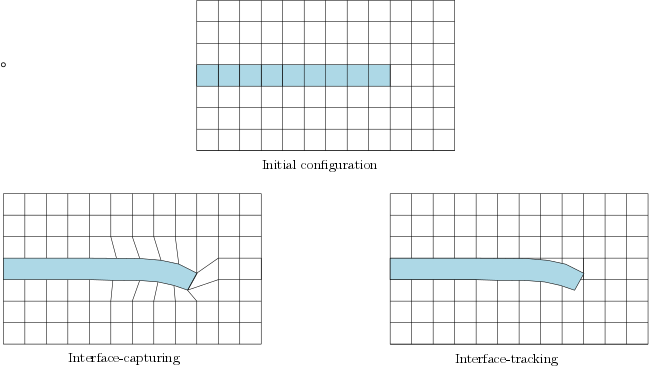
\includegraphics[scale=0.5]{./Fig/interface.png}
      \caption{Comparison of interface-tracking and interface-capturing for an elastic beam undergoing deformation}
\end{figure}

Among the multiple approaches within CFSI, the arbitary Lagrangia-Eulerian methos is chosen for this thesis. 



%We define $\Omega$ in the \textit{reference configuration} be partitioned in a fluid domain $\hat{\Omega_f}$ and a structure domain $\hat{\Omega_s}$ such that
%$\Omega = \hat{\Omega_f} \cup \hat{\Omega_s}$. Further we define the interface $\hat{\Gamma}$ as the interface between these domains such that $\Gamma_i = \hat{\partial \Omega_f} \cap \hat{\partial %\Omega_s}$. 
%The fluid-structure interaction problem is then defined by the fluid and solid equations, and the transmission of the \textit{kinematic} and \textit{dynamic} conditions on the interface $\hat{\Gamma}$. 


%\section{Fully Eulerian}
%This method keeps the fluid in its \textit{Eulerian coordinates}, and such can be seen as the natural counterpart of the ALE method \cite{Wick2013}. First proposed by , \cite{Dunne2006}. One motivation of such and approach is the handling of large-deformation, as the transformation to eulerian coordinates are purely natural.

\section{Arbitary Lagrangian Eulerian formulation}
The \textit{arbitary Lagrangian-Eulerian} formulation is the most popular approach within \textit{Interface-tracking} \cite{Richter2010a}, \cite{Frei2016}, initially developed to combine the strengths of the \textit{Lagranngian} and \textit{Eulerian} coordinate systems. In this approach the structure is given in its natural \textit{Lagrangian coordinate system}, while transforming the fluid domain into an artificial coordinate system similar to the \textit{Lagrangian coordinate system}. Since no natural displacement occur in the fluid domain, the transformation has no directly physical meaning \cite{Richter2010a}, \cite{Donea2004}. 
 
With this in mind, we will derive these transformations with the help of a new arbitary fixed reference system \ha{W}, following the ideas and approaches found in \cite{Richter2016}. Further we denote its deformation gradient as $\hat{F}_w$ and its determinant $\ha{J}_w$. Following the ideas from chapter 2, we introduce the invertibale mapping $\ha{T}_w : \ha{W} \rightarrow V(t)$ , with the scalar $\ha{f}(\ha{x}_W, t) = f(x,t) $ and vector $\hat{w}(\ha{x}_W, t) = \mathbf{w}(x,t) $ counterparts.\\ 
For $\ha{V} = \ha{W}$, $\ha{W}$ simply denotes the familiar Lagrangian description.
In the case $\ha{V} \neq \ha{W}$, $\ha{W}$ as pointed out earlier have no direct physical meaning.  Hence it is important to notice that the physical velocity $\hat{v}$ and the velocity of arbitrary domain $\pder{\ha{W}_w}{t}$ doesn't necessary coincide. This observation is essential, as we will soon see. \\

We will first define the transformation of spatial and temporal derivatives from $V(t)$ to $\ha{W}$ found in \cite{Richter2016}\\

\begin{lem}
Transformation of scalar spatial derivatives \\
\textit{Let f be a scalar function such that} $f: V(t) \rightarrow \mathbb{R}$, \textit{then} 
\begin{align}
\nabla f = \hat{F}_W^{-T} \hat{\nabla}\ha{f}
\end{align} 
\end{lem}

\begin{lem}
Transformation of vector spatial derivatives \\
\textit{Let \textbf{w} be a vector field such that} $\mathbf{w}: V(t) \rightarrow \mathbb{R}^d$, \textit{then} 
\begin{align}
\nabla \mathbf{w} = \hat{\nabla}\hat{w} \hat{F}_W^{-1} 
\end{align} 
\end{lem}

\begin{lem}
Transformation of scalar temporal derivatives \\
\textit{Let f be a scalar function such that} $f: V(t) \rightarrow \mathbb{R}$, \textit{then} 
\begin{align}
\pder{f}{t} = \pder{\ha{f} }{t} - (\hat{F}_W^{-1} \pder{\ha{T}_W}{t} \cdot \hat{\nabla}) \ha{f}
\end{align} 
\end{lem}

In addition we need a consistent way to transform the induced stresses in the \textit{Eulerian} coordinate system to $\ha{W}$. Hence we introduce the \textit{Piloa transformation}, found in most introduction courses in structure mechanics.
\\
\begin{lem}
T \\
\textit{Let \textbf{w} be a vector field such that} $\mathbf{w}: V(t) \rightarrow \mathbb{R}^d$, \textit{then the Piola transformation of w is defined by} 
\begin{align}
\mathbf{w} = \ha{J}_W \hat{F}^{-1}_W \hat{w}
\end{align} 
\end{lem}

The Piola transformation can be further extended to transform tensors, see \cite{Richter2016}, Orange book. This results is essential as it allows us to transform surface forces induced by the \textit{Cauchy stress tensor} on our arbitrary coordinate system $\ha{W}$. Lemma 1.4 brings us to \textit{the first Piola Kirchhoff stress tensor} $\hat{P} = \ha{J}_W \hat{\sigma}\hat{F}_W^{-T}$.

\subsection{ALE formulation of the fluid problem}

Recall the Navier-Stokes equation defined in the \textit{Eulerian coordinate system} V(t).
\begin{align*}
&\rho \pder{\mathbf{v}}{t} + \rho \mathbf{v} \cdot \nabla \mathbf{v} =
\nabla \cdot \sigma + \rho \mathbf{f} \\
&\nabla \cdot \mathbf{v} = 0
\end{align*}
Using our newly introduced transformations of derivatives we map the equation to the arbitrary reference system $\ha{W}$. We will first consider the transformation of the\textit{material derivative}. By 
\begin{align*}
\frac{d \mathbf{v}}{dt}(x,t) = \pder{\mathbf{v}}{t}(x,t) + \nabla \mathbf{v}(x,t) \cdot \pder{x}{t} \\
\frac{d \mathbf{v}}{dt}(x,t) = \pder{\mathbf{v}}{t}(x,t) + \nabla \mathbf{v}(x,t) \cdot \mathbf{v}
\end{align*}
Note $\pder{x}{t}$ is the velocity of particles and not the transformation velocity $\pder{\ha{T}_W}{t}$. By lemma(1.1, 1.2, 1.3) we have  

\begin{align*}
\frac{d \mathbf{v}}{dt}(x,t) = 
\pder{\hat{v}}{t}(x,t) - (\hat{F}_W^{-1}\pder{\ha{T}_W}{t} \cdot \hat{\nabla})\hat{v}
+ \hat{F}_W^{-T}\hat{\nabla}\hat{v} \cdot \hat{v} \\
\mathbf{v} \cdot \nabla \mathbf{v} = \nabla \mathbf{v} \mathbf{v} = 
\hat{\nabla}\hat{v}\hat{F}_W^{-1}\hat{v} = (\hat{F}_W^{-1}\hat{v} \cdot \hat{\nabla})\hat{v} \hspace{4mm} \textit{FINN KILDE}
\end{align*}

These results can be used to show that

\begin{align*}
\pder{\mathbf{v}}{t} + \mathbf{v} \cdot \nabla \mathbf{v} =
\pder{\hat{v}}{t} + (\hat{F}_W^{-1}(\hat{v} - \pder{\ha{T}_W}{t}) \cdot \hat{\nabla}) \hat{v}
\end{align*}

By applying \textit{the first Piola Kirchhoff stress tensor} directly we transform the surface stress by 

\begin{align*}
\nabla \cdot \sigma = \nabla \cdot (\ha{J}_W \hat{\sigma}\hat{F}_W^{-T})
\end{align*}
In general, $\sigma$ is presumed on the form of a Newtonian fluid.
However special care must be taken, as $\sigma \neq \hat{\sigma}$ due to spatial derivatives within the tensor. Hence 
\begin{align*}
\sigma = -p I + \mu_f(\nabla \mathbf{v} + (\nabla \mathbf{v})^T \\
\hat{\sigma} = -\ha{p} I + \mu_f(\hat{\nabla}\hat{v}\hat{F}_W^{-1} +\hat{F}_W^{-T}\hat{\nabla}\hat{v}^T )
\end{align*} 

For the conservation of continuum we apply the \textit{Piola Transformation} such that

\begin{align*}
\nabla \cdot \mathbf{v} = \nabla \cdot (\ha{J} \hat{F}_W^{-1} \hat{v})
\end{align*}

\subsection{ALE formulation of the solid problem}

With the introduced mapping identities we have the necessary tools to derive a full fluid-structure interaction problem defined of a fixed domain. Since the structure already is defined in its natural Lagrangian coordinate system, no further derivations are needed for defining the total problem.

\begin{equat}
\textit{ALE problem on a fixed domain}
\begin{align}
\ha{J} \pder{\hat{v}}{t} + \ha{J} (\hat{F}_W^{-1}(\hat{v} - \pder{\ha{T}_W}{t}) \cdot \hat{\nabla}) \hat{v}
= \nabla \cdot (\ha{J}_W \hat{\sigma}\hat{F}_W^{-T}) + \rho_f \ha{J} \mathbf{f}_f
\hspace{4mm} \text{in} \hspace{2mm} \Omega_f \\
\nabla \cdot (\ha{J} \hat{F}_W^{-1} \hat{v}) \hspace{4mm} \text{in} \hspace{2mm} \Omega_f \\
\rho_s \pder{\hat{v}_s}{t} = \nabla \cdot \mathbf{F}\mathbf{S} + \rho_s \mathbf{f}_s
\hspace{4mm} \text{in} \hspace{2mm} \Omega_s \\
\pder{\hat{v}_s}{t} = \hat{u}_s \hspace{4mm} \text{in} \hspace{2mm} \Omega_s \\
\hat{v}_s = \hat{v}_f \hspace{4mm} \text{on} \hspace{2mm} \Gamma_i \\
\ha{J}_W \hat{\sigma}\hat{F}_W^{-T} \cdot \mathbf{n} = 
\mathbf{F}\mathbf{S} \cdot \mathbf{n}  \hspace{4mm} \text{on} \hspace{2mm} \Gamma_i 
\end{align}
\end{equat}


\subsection*{Fluid mesh movement}
In the ALE framwork one of the most limiting factors is the degeneration of the mesh due to large deformations. Even the most advanced ALE formulated schemes reaches a limit when only re-meshing is nesecarry \cite{Wall12006}. Consequently the choice of an appropriate mesh moving technique is essential to preserve a feasible mesh quality for the simulation of fluid flow. Let the total domain deformation $\ha{T}(\ha{x}, t)$ be divided into the solid and fluid deformation $T_s$, $T_f$, were the fluid deformation is mapped to the arbitrary fixed reference system $\ha{W}$ presented in the last subsection.  
Then the ALE map $T_f$ on the form 
\begin{align*}
\ha{T}_f(\ha{x}, t) = \hat{x} + \hat{u}_f(\hat{x}, t)
\end{align*}
is constructed such that $\hat{u}_f$ is an extension of the solid deformation $\hat{u}_s$ from the interface to the fluid domain. Several extentions have been proposed throuhout the litteratur, and for an overview the reader is refered to \cite{MM2016}, and the reference therein. The construction of such extensions often involves solving some auxiliary problem on a partial differential equation(PDE) form, mainly of second-order. The \textit{Laplacian} and \textit{pseudo-elasticity} extentions are examples, which will be considered in this thesis. These extensions are beneficial in terms of simplicity and computational efficiency, but comes with a cost of user mesh customization. One often want to ensure a desired mesh position and some regularity of mesh spacing on the boundary, but it is impossible for second order extensions to specify both \cite{Helenbrook2003}. Therefore the author of \cite{Helenbrook2003}, proposes a fourth-order PDE, the \textit{biharmonic} extensions, to improve the regularity of the mesh deformation. \\

\subsubsection*{Laplacian model}

The main motivation for a \textit{Laplacian} smoothing is due to its simplicity and due to its property of bounding the interior displacements to the boundary values. 

\begin{align*}
&- \hat{\nabla} \cdot (\alpha^q \hat{\nabla} \hat{u}) = 0 \\
&\hat{u}_f = \hat{u}_s \hspace{2mm} \text{on} \hspace{2mm}  \Gamma \\
&\hat{u}_f = 0 \hspace{2mm} \text{on} \hspace{2mm} \partial \hat{\Omega}_f / \Gamma 
\end{align*}

Most favourable, the largest mesh deformation occuring should be confined to the interal part of the mesh as it causes the least distortion \cite{Jasak2006}. Therefore the introduced diffusion parameter $\alpha$, often raised to some power q, is introduced to manipulate this behaviour. The form of this paramter is often problem specific,  as selective treatment of the elements may vary from different mesh deformation problems. A jacobian based method was introduced in \cite{Stein}. In \cite{Jasak2006}, the authors reviewed several distance based options, where $\alpha$ was some function of the distance to the closest moving boundary. This method was adopted in this thesis on the form

\begin{align*}
\alpha(x) = \frac{1}{x^q}  \hspace{4mm} q = -1
\end{align*}

However as pointed out by \cite{Hsu}, one of the main disadvantages of using the linear Laplace equation is that the equation solves the mesh deformation components independently of one another. Say one have deformation only in the x-coordinate direction, the interior mesh points will only be moved along this deformation. Such a behavior restricts the use to the Laplace equation of mesh extrapolation purposes.

\subsubsection*{Linear elastic model}
Considering a linear elastic model for mesh moving was first introduced in \cite{Tezduyar1992}.  
Both \cite{Dwight}
\begin{align*}
&\nabla \cdot \sigma = 0 \\
&\sigma = \lambda Tr(\epsilon(u)) I + 2 \mu \epsilon(u) \\
&\epsilon(u) = \frac{1}{2}(\nabla u + \nabla  u^T)
\end{align*}

Where Lamé constants $\lambda$ and $\nu$ are given as

\begin{align*}
\lambda = \frac{\nu E}{(1 + \nu)(1 - 2\nu)} \hspace{2mm} \mu = \frac{E}{2(1 + \nu)}
\end{align*}

One of the main motivations for introducing such a model is the manipulation of Young's modulus $E$, and the poisson´s ration $\nu$. Recall that Young's modulus is the measurement of the a materials stiffness, while the poission's ratio describe the materials stretching in the transverse direction under extension in the axial direction. Manipulating these parameters one can influence the mesh deformation,
however the choice of these parameters have proven not to be consistent,  and to be dependent of the given problem.  \\

In \cite{Wicka} the author proposed a negative possion ratio, which makes the model mimic an auxetic material. Such materials becomes thinner in the perpendicular direction when they are submitted to compression, and this property is feasible for mesh under deformation. 

One of the most common approach is to set $\nu$ as a constant in the range $\nu \in [0, 0.5)$ and let $E$ be the inverse of the distance of an interior node to the nearest boundary surface \cite{MM2016}. 
The authors of \cite{Biedron} used this property and also argued that the Young's modulus also could be chosen as the inversely proportional to the cell volume. They also pointed out that both approaches would give the desired result that the small cells around the solid surface would modeled rigid, moving with the surface of the solid as it undergoes deformation. On the other hand cells further away will deform to counter the effects close to the solid surface.

\subsubsection*{Biharmonic model}
Using a biharmonic mesh deformation model provides further freedom in terms of boundary conditions, and the reader is encoured to consult \cite{Helenbrook2003} for a deeper review. We will in combination with \cite{Wicka} present two main approaches the biharmonic model is defined as 
\begin{align*}
\hat{\nabla}^2 \ha{u} = 0 \hspace{4mm} \text{on} \hspace{2mm} \hat{\Omega}_f 
\end{align*}
By introducing a second variable on the form $\ha{w} = - \hat{\nabla} \ha{u}$, we get the following system defined by 
\begin{align*}
&\hat{w} = -\hat{\nabla}^2\hat{u} \\
&- \hat{\nabla} \hat{w} = 0
\end{align*}

This model is defined in a mixed formulation, and as such the prize for quality and control of mesh deformation comes with the cost of more computational demanding problem. 

For the boundary conditions two types has been proposed in \cite{Wicka}. Let 
$\hat{u}_f$ be decomposed by the components $\hat{u}_f = (\ha{u}_f^{(1)}. \ha{u}_f^{(2)})$. Then we have

\begin{align*}
&\textbf{Type 1} \hspace{4mm} \ha{u}_f^{(k)} = \pder{\ha{u}_f^{(k)}}{n} = 0 \hspace{4mm} \partial \hat{\Omega}_f / \Gamma \hspace{2mm} \text{for} \hspace{1mm} k = 1, 2 \\
&\textbf{Type 2} \hspace{4mm} \ha{u}_f^{(1)} = \pder{\ha{u}_f^{(1)}}{n} = 0 
\hspace{2mm} \text{and} \hspace{2mm} \ha{w}_f^{(1)} = \pder{\ha{w}_f^{(1)}}{n} = 0 \hspace{4mm} \text{on} \hspace{1mm} \hat{\Omega}_f^{in} \cup \hat{\Omega}_f^{out} \\ 
&\hspace{17mm}  \ha{u}_f^{(2)} = \pder{\ha{u}_f^{(2)}}{n} = 0 
\hspace{2mm} \text{and} \hspace{2mm} \ha{w}_f^{(2)} = \pder{\ha{w}_f^{(2)}}{n} = 0 \hspace{4mm} \text{on} \hspace{1mm}  \hat{\Omega}_f^{wall}
\end{align*}

With the first type of boundary condition the model can interpreted as the bending of a thin plate, clamped along its boundaries. The form of this problem has been known since 1811, and its derivation has been connected with names like  French scientists Lagrange, Sophie Germain, Navier and Poisson \cite{Meleshko1997}.  

The main motivation for second type of boundary condition is for a rectangular domain where the coordinate axes match the Cartesian coordinate system \cite{Wicka}. In such a configuration, the mesh movement is only constrained in the perpendicular direction of the fluid boundary, leading to mesh movement in the tangential direction. This special case reduces the effect of distortion of the cells.  

\newpage

\newpage
\section{Discretization of the FSI problem}
Say something general of FSI discretization.. FEM, FVM, ...
In this thesis, the finite element method will be used to discretize the coupled fluid-structure interaction problem. It is beyound of scope  of this thesis, to thorough dive into the analysis of the finite element method regarding fluid-structure interaction problems. Only the basics of the method, which is nesecarry in order to define a foundation for problem solving will be introduced. 

\subsection{Finite Element method}
Let the domain $\Omega(t) \subset \mathbb{R}^d \ (d = 1, 2, 3) $  be a time dependent domain discretized a by finite number of d-dimentional simplexes.  Each simplex is denoted as a finite element, and the union of these elements forms a mesh. Further, let the domain be divided by two time dependent subdomains $\Omega_f$ and $\Omega_s$, with the interface $\Gamma = \partial \Omega_f \cap \partial \Omega_s$. The initial configuration $\Omega(t), t = 0 $ is defined as $\hat{\Omega}$, defined in the same manner as the time-dependent domain. $\hat{\Omega}$ is  known as the \textit{reference configuration}, and hat symbol will refer any property or variable to this domain unless specified. The outer boundary is set by $\partial \hat{\Omega}$ , with $\partial \hat{\Omega}^D$ and $\partial \hat{\Omega}^N$ as the Dirichelt and Neumann boundaries respectively. \\ \\

The family of Lagrangian finite elements are chosen, with the function space notation,
\begin{align*}
\hat{V}_{\Omega} := H^1(\Omega) \hspace{4mm} 
\hat{V}_{\Omega}^0 := H_0^1(\Omega)  
\end{align*}
where $H^n$ is the Hilbert space of degree n. \\
Let Problem 2.1 denote the strong formulation. By the introduction of appropiate trial and test spaces of our variables of interest, the weak formulation can be deduced by multiplying the strong form with a test function and taking integration by parts over the domain.  This reduces the differential equation of interest down to a system of linear equations. (skriv bedre..) \\
The velocity variable is continous through the solid and fluid domain
\begin{align*}
\hat{V}_{\Omega, \gat{v}} := \gat{v} \in H_0^1(\Omega), \hspace{2mm} 
\gat{v}_f = \gat{v}_s \ \text{on} \ \hat{\Gamma}_i \\
\hat{V}_{\Omega, \gat{\psi}} := \gat{\psi}^u \in H_0^1(\Omega), \hspace{2mm} 
\gat{v}_f = \gat{v}_s \ \text{on} \ \hat{\Gamma}_i 
\end{align*}
For the deformation, and the artificial deformation in the fluid domain let
\begin{align*}
\hat{V}_{\Omega, \gat{v}} := \gat{u} \in H_0^1(\Omega), \hspace{2mm} 
\gat{u}_f = \gat{u}_s \ \text{on} \ \hat{\Gamma}_i \\
\hat{V}_{\Omega, \gat{\psi}} := \gat{\psi}^v \in H_0^1(\Omega), \hspace{2mm} 
\gat{\psi}_f^v = \gat{\psi}_s^v \ \text{on} \ \hat{\Gamma}_i 
\end{align*}

For simplification of notation the inner product is defined as
\begin{align*}
\int_{\Omega} \gat{v} \ \gat{\psi} \ dx = (\gat{v}, \ \gat{\psi})_{\Omega}
\end{align*}
 

\subsection{Variational Formulation}
With the primaries set, we can finally define the discretization of the monolithic coupled fluid-structure interaction problem. For full transparency, variation formulation of all previous suggested mesh motion models will be shown. For brevity, the laplacian and linear elastic model will be shorted such that 
\begin{align*}
&\hat{\sigma}_{\text{mesh}} = \alpha \nabla \mathbf{u} \hspace{2mm} \text{Laplace} \\
&\hat{\sigma}_{\text{mesh}} =  \lambda Tr(\epsilon(\mathbf{u})) I + 2 \mu \epsilon(\mathbf{u}) \hspace{2mm} \text{Linear Elasticity} 
\end{align*}
Further, only the biharmonic model for the first type of boundary condition will be introduced as the second boundary condition is on a similar form.
  By the concepts of the Finite-element method, the weak variation problem yields.

\begin{prob}
\textit{Coupled fluid structure interaction problem for laplace and elastic mesh moving model.
Find $\bat{u}_s, \bat{u}_f, \bat{v}_s, \bat{v}_f, \ha{p}_f $ such that}
\begin{align*}
\big(\ha{J} \pder{\bat{v}}{t}, \ \gat{\psi}^u \big)_{\hat{\Omega}_f} +
\femf{\ha{J} (\hat{F}_W^{-1}(\bat{v} - \pder{\ha{T}_W}{t}) \cdot \hat{\nabla}) \bat{v}}{\gat{\psi}^u}
+ \femi{\ha{J}_W \hat{\sigma}\hat{F}_W^{-T} \bat{n}_f}{\gat{\psi}^u} \\
- \femf{\ha{J}_W \hat{\sigma}\hat{F}_W^{-T}}{\hat{\nabla}\gat{\psi}^u} -
\femf{\rho_f \ha{J} \mathbf{f}_f}{{\gat{\psi}^u}} = 0 \\
\fems{\rho_s \pder{\bat{v}_s}{t}}{\gat{\psi}^u} + \femi{\bat{F}\bat{S}\bat{n}_f}{\gat{\psi}^u}
- \fems{\bat{F}\bat{S}}{\nabla \gat{\psi}^u} - \fems{\rho_s \bat{f}_s}{\gat{\psi}^u} = 0 \\
\fems{\pder{\bat{v}_s - \bat{u}_s}{t}}{\gat{\psi}^v}  = 0\\
\femf{\nabla \cdot (\ha{J} \hat{F}_W^{-1} \bat{v})}{\gat{\psi}^p} = 0 \\
\femf{\hat{\sigma}_{\text{mesh}}}{\hat{\nabla}\gat{\psi}^u} = 0
\end{align*} 
\end{prob}

\begin{prob}
\textit{Coupled fluid structure interaction problem for biharmonic mesh moving model.
Find $\bat{u}_s, \bat{u}_f, \bat{v}_s, \bat{v}_f, \ha{p}_f $ such that}
\begin{align*}
\big(\ha{J} \pder{\bat{v}}{t}, \ \gat{\psi}^u \big)_{\hat{\Omega}_f} +
\femf{\ha{J} (\hat{F}_W^{-1}(\bat{v} - \pder{\ha{T}_W}{t}) \cdot \hat{\nabla}) \bat{v}}
{\gat{\psi}^u}
+ \femi{\ha{J}_W \hat{\sigma}\hat{F}_W^{-T} \bat{n}_f}{\gat{\psi}^u} \\
- \femf{\ha{J}_W \hat{\sigma}\hat{F}_W^{-T}}{\hat{\nabla}\gat{\psi}^u} -
\femf{\rho_f \ha{J} \mathbf{f}_f}{{\gat{\psi}^u}} = 0 \\
\fems{\rho_s \pder{\bat{v}_s}{t}}{\gat{\psi}^u} + \femi{\bat{F}\bat{S}\bat{n}_f}{\gat{\psi}^u}
- \fems{\bat{F}\bat{S}}{\nabla \gat{\psi}^u} - \fems{\rho_s \bat{f}_s}{\gat{\psi}^u} = 0 \\
\fems{\pder{\bat{v}_s - \bat{u}_s}{t}}{\gat{\psi}^v}  = 0\\
\femf{\nabla \cdot (\ha{J} \hat{F}_W^{-1} \bat{v})}{\gat{\psi}^p} = 0 \\
\femf{\hat{\nabla}\bat{u}}{\hat{\nabla}\gat{\psi}^{\eta}} - 
\femf{\bat{w}}{\hat{\nabla}\gat{\psi}^u} = 0 \\
\femf{\hat{\nabla}\bat{w}}{\hat{\nabla}\gat{\psi}^{v}} = 0
\end{align*}
\text{for the first type of boundary conditions introduced. } 
\end{prob}

Both problems introduced must handle the \textit{kinematic} and \textit{dynamic} boundary conditions in a consistent way. By a continuous velocity field on the whole domain, the \textit{kinematic} condition is strongly enforces on the interface $\hat{\Gamma}_i$
The continuity of normal stresses on the interface are defined as
\begin{align*}
 \femf{\ha{J}_W \hat{\sigma}\hat{F}_W^{-T} \bat{n}_f}{\gat{\psi}^u} = 
  \fems{\bat{F}\bat{S} \bat{n}_s}{\gat{\psi}^u}
\end{align*}
This condition is weakly imposed by omitting the boundary integral from the variational formulation \cite{Wick}, and it becomes an implicit condition for the system. \\

\newpage
\chapter{Verification and Validation}
 Computer simulations are in many engineering applications a cost-efficient way of conducting design and performance optimalization of physical problems. But blindly trusting numbers generated from a computer code can prove to be naive. It doesn't take a lot of coding experience before one realizes many things that can brake down and produce unwanted or unexpected results. 
Therefore, \textit{credability} of computational results are essential, meaning the simulation is worthy of belief or confidence \cite{Oberkampf2010}. \textit{Verification and validation} (V\&V) is the main approach for assessing the reliability of computational simulations \cite{Sommerville2006}.  A thorough discussion  of (V\&V) concepts and terminology can be found in \cite{Oberkampf2010}. In this thesis, the definitions provided by the \textit{American Society of Mechanical Engineers guide for Verification and Validation in Computational Solid Mechanics}  \cite{Schwer2006} are followed:

\begin{defn}
Verification: The process of determining that a computational model accurately represents
the underlying mathematical model and its solution. 
\end{defn}

\begin{defn}
Validation: The process of determining the degree to which a model is an accurate
representation of the real world from the perspective of the intended uses of the model. 
\label{eq:intcond}
\end{defn}

Simplified, \textit{verification} considers if one solves the equations right, while \textit{validation} is checking if one solves the right equations for the given problem \cite{Roache}. To test a computational code for all possible parameters, conditions, and applications, are simply too time consuming. Verification and validation is therefore ongoing processes, with no clear boundary of completeness unless additional requirements are specified \cite{Roache}. The goal of this chapter is to verify the implementations using the method of manufactured solution  (MMS), addressing validation in a subsequent chapter.

\section{Verification of Code}
Within scientific computing a mathematical model is often the baseline for simulations of a particular problem of interest. For scientists exploring physical phenomena, the mathematical model is often on the form of systems of partial differential equations (PDEs). 
Through verification of code, the ultimate goal is to ensure a computer program truly represents the mathematical model. To accumulate sufficient evidence that a mathematical model is solved correctly by a computer code,  it must excel within predefined criteria. If the acceptance criterion is not satisfied, a coding mistake is suspected. Should the code pass the preset criteria, the code is considered verified. Of the different classes of test found in \cite{Roache},  \textit{Order-of-accuracy} (OAA)  is regarded as the most rigorous acceptance criterion for verification \cite{Biggs, Roache, Etienne2006}. The method tests if the discretization error $E$ is reduced in coordinance with the \textit{formal order of accuracy} expected from the numerical scheme. The formal order of accuracy is defined to be the theoretical rate at which the truncation error of a numerical scheme is expected to reduce. The \textit{observed order of accuracy} is the actual rate produced by the numerical solution. For order of convergence tests, the code is assumed to be verified if the observed discretization error is proportional to the formal order of accuracy.  Monitoring the dicretization error $E$ by spatial and temporal refinements, one assumes the error $E$ can be expressed as,

\begin{align*}
&E = C\Delta t^p + D\Delta x^l\\
\end{align*} 
where C and D are constants, $\Delta t$ and $\Delta x$ represents the spatial and temporal resolution, while $p$ and $l$ is the observed order of accuracy of the numerical scheme. If $\Delta x$is small compared to $\Delta t$, the spatial discretization error can be neglected, which can use that to find $l$, which is the observed order of convergence for the temporal discretization error. To calculate the error, $E$, an exact/reference solution is needed which rarely exist for complex mathematical models. The next subsection presents an efficient method for generating such solutions.

\subsection{Method of manufactured solution}
The basis of a convergence test is to find an exact/reference solution,  to compute the discretization error $E$. However, solutions of PDEs are limited, and simplifications of the original problem are often necessary to produce analytical solutions. \textit{The method of manufactured solutions} provides a simple yet robust way of making analytic solutions for PDEs. 
Let a  partial differential equation of interest be on the form
\begin{align*}
\textbf{L}(\textbf{u}) = \textbf{f}
\end{align*}

Here \textbf{L} is a differential operator, \textbf{u} is variable the of interest, and \textbf{f} is some sourceterm. In MMS, one first manufactures a solution \textbf{u} for the given problem, producing a sourceterm  \textbf{f} after differentiation by \textbf{L}. The produced source term will cancel any imbalance formed by the manufactured solution \textbf{u} of the original problem. Therefore, the manufactured solution can be constructed without any physical reasoning, proving code verificaion as a purely a mathematical exercise were the only interest is to verify the solution \cite{Roache2002}. 
\newpage
If the MMS is not chosen properly, the test will not work. Therfore some guidelines for rigirous verification have been proposed in \cite{Etienne2006, Biggs, Roache2002}:

\begin{itemize}
\item The manufactured solution (MMS), should be composed of smooth analytic functions such as exponential, trigonometric, or polynomials.
\item The MS should should have sufficient number of derivatives, exercising all terms and derivatives of the PDEs. 
\end{itemize}

To properly verify the robustness of the method of manufactured solution, a report regarding code verification through  MMS for the time-dependent Navier-Stokes equation was published by Salari and Knupp \cite{Biggs}.  To prove its robustness, the authors deliberate implemented  code errors in a verified Navier-Stokes solver through MMS. In total 21 blind test-cases where implemented, where different approaches of verification frameworks were tested.  Of these, 10 coding mistakes that reduced the observed order-of-accuracy was implemented. The MMS captured all coding mistakes, except one. This mistake would, accordingly to the author, been captured if his guidelines for conducting MMS had been followed. \\

In general, computing the source term $\mathbf{f}$ can be quite challenging and error prone.  Therefore, symbolic computation of the sourcterm is advantageous to overcome mistakes which can easily occur when calulating by hand. For construction of the sourceterm \textbf{f}, the Unified Form Language (UFL) \cite{Alnes2015} provided in FEniCS Project will be used. COMPUTE VV HERE

\subsection{Comment on verification of the fluid-structure interaction solver by MMS}
In general the MMS does not need to match any physical processes. However, when considering multiphysics problems, such as FSI, the equations has to meet the mathematical criteria from Section ~\ref{sec:intcond}: \\

\textit{Let $\bat{v}_s, \bat{v}_f$ be the structure and fluid velocity, and let $\sigma_s$, $\sigma_f$ be the Cauchy stress tensor for the structure and fluid respectively. Let $\mathbf{n}_i$ be the normal vector pointing out of the domain $i$. We then have the following interface boundary conditions.}:
\begin{enumerate}
\item Kinematic boundary condition $\bat{v}_s = \bat{v}_f$, enforced strongly by a continuous velocity field in the fluid
        and solid domain.
\item Dynamic boundary condition $\sigma_s \cdot \mathbf{n}_s = \sigma_f \cdot \mathbf{n}_f$, enforced weakly by omitting the 
        boundary integrals from the weak formulation in problem.
\end{enumerate}
The choice of a MMS is therefore not trivial, as it must fulfill condition 1 and 2, in addition to the divergence-free condition in the fluid, and avoiding cancellation of the ALE-convective term $\pder{\hat{T}_f}{t}$.  The construction of a MMS for a monolithic FSI problem is therefore out of the scope of this thesis. The struggle is reflected of the abscence of research, regarding MMS for coupled FSI solvers in the litterature. The challenge is often disregarded, such as \cite{Sheldon2014}, where the verification process is conducted on the fluid and structure solver separately. Instead, the accuracy of the coupling is evaluated by the code validation. The approach clearly ease the process, assuming verification of each codeblock is "sufficient" to declare the code verified. In this thesis, the approach found in \cite{Sheldon2014} was followed, but it must be stressed that solving each problem individually is not true verification, in reference to a monolithic approach where the problems are simultaneously.

\section{Validation of Code}
Through \textit{verification}, one can assure that a scientific code evaluate mathematical model correctly. However, accuracy is unnecessary if the model fails to serve as an appropriate representation of the physical problem. By definition ~\ref{eq:intcond}, \textit{Validation} is the act of demonstrating that a mathematical model is applicable for its intended use with a certain degree of accuracy. That is, a mathematical model is validated if it meets some predefined criteria within a specific context. Validation is therefore not intended to portray the model as an absolute truth, nor the best model available \cite{Rykiel1996}. In scicomp., validation is conducted by comparing numerical results against existing experimental data. The design of validation experiments vary by the motivation of the of their creators, where validated experiments for computational science can be divided into three groups \cite{Sommerville2006}: (1)To improve fundamental understanding of a physical process, (2)Discovery or enhancement of mathematical models of well known physical processes, (3)To conclude the reliability and performance of systems. The assessment of comparison between numerical results and experimental data, makes \textit{validation} assess a wide range of issuses \cite{Sommerville2006}. Is the experiment relevant, and  conducted correctly in accordinance with prescribed parameters? What about the measurement uncertainty of reference experimental data? These issues  must be addressed in order to raise sufficient confidence that the mathematical model is credible for its intended use. \\


 \newpage
 
\section{Validation benchmark}
The numerical benchmark presented in \cite{Hron2006} has been chosen for validation of the \textit{One-step $\theta$} scheme from chapter 3. The benchmark has been widely accepted as a rigid validation benchmark  throughout the litterature \cite{Wickb, Wick, V2013, Gatzhammer2014}. This is mainly due to the diversity of tests included, challenging all the main components of a fluid-structure interaction scheme. The benchmark is based on the \textit{von Kármán vortex street} \cite{White}, where a cylinder is placed off-center in a 2D channel. In \cite{Hron2006}, an additional elastic flag is placed behind the cylinder, see Figure 4.1

\begin{figure}[h!]
  \centering
    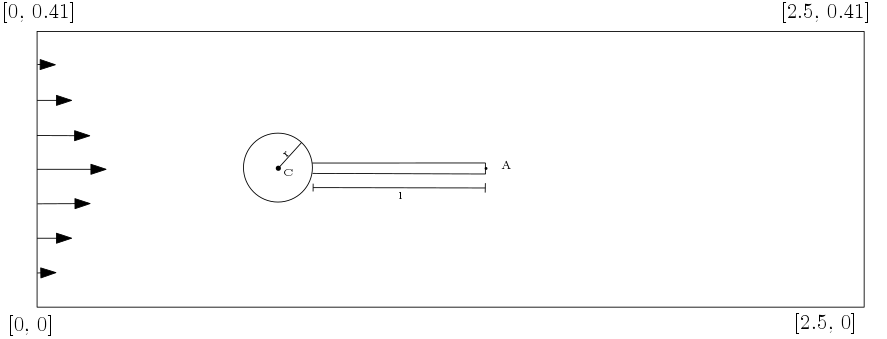
\includegraphics[scale=0.2]{./Fig/turekflag.png}
      \caption{Computational domain of the validation benchmark}
      \label{fig:tflag}
\end{figure}

The benchmark is divided into three problems, each further divided into three different sub-problems with increasing complexity. In the first problem, the fluid solver is tested for a series of different flow profiles. The second branch considers the structure solver, regarding bending of the elastic flag. And the final branch concerns validation of a full fluid-structure interaction problem with the fluid and the elastic flag .  Several quantites for comparion are presented in \cite{Hron2006} for validation purposes:

\begin{itemize}
\item The position (x,y) of point A(t) as the elastic flag undergoes deformation.
\item Drag and lift forces exerted on of the whole interior geometry in contact with the fluid, consisting of the rigid circle and the elastic beam.
\begin{align*}
(F_D, F_L) = \int_{\Gamma} \mathbf{\sigma} \cdot \mathbf{n} dS
\end{align*}
\end{itemize}

\newpage
All problems pose both steady state and periodic solutions. For the steady state solutions, the quantity of interest will be calculated based on a transient simulation, that has converged towards a steady state solution. For the periodic solutions, the amplitude and mean values for the time dependent quantity are calculated from the last period.
\begin{align}
\text{mean} = \frac{1}{2} \text{max + min} \\
\text{amplitude} = \frac{1}{2} \text{max - min}
\label{icond}
\end{align}
 In \cite{Hron2006}, all steady state solutions seems to be calulated by solving a steady state equation since time-step are only reported for the periodic solutions. In this thesis, all problems in \cite{Hron2006} are calculated using time integration. The main reason for solving the problem transiently rather than steady state, is that numerical errors associated with initial transients are negligible with a sufficiently low time step size, without laborious changes to the numerical implementation. In the following section, an overview of each problem together with numerical results will be presented. A  discussion of the results are given at the end of each simulation brancht. For each table, the relative error of the finest spatial and temporal refinement compared to the reference solution is reported in \cite{Hron2006}.

\subsection{Validation of fluid solver}
The validation of the fluid solver concerns transient flow for a low Reynold-number regime. Two approaches for the validation are given in \cite{Hron2006}. The first approach considers the setup as a fluid-structure interaction problem, setting the elastic flag close to rigid by manipulation of the structure parameters. In the second approach, the flag is set fully rigid and considered a purely flow problem, meaning any influence of the structure and mesh moving model is eliminated.  Hence, no deformation of the fluid domain occurs, and the fluid problem can be defined in an Eulerian description of motion.  \\

\textit{Let $\mathbf{v}_f$, ${p}_f$ be the fluid velocity and pressure, and let  $\sigma_f$ be the Cauchy stress tensor, and $\mathbf{f}_f$ denote any sourceterm,  Find $\mathbf{v}_f$, ${p}_f$ such that }:
\begin{align*}
 \big( \pder{\mathbf{v}_f}{t}, \ \bm{\psi}^u \big)_{\hat{\Omega}_f} +
\feme{(\mathbf{v}_f \cdot \nabla) \mathbf{v}_f}{\bm{\psi}^u}
- \feme{\hat{\sigma}}{\nabla\bm{\psi}^u} -
\feme{\rho_f  \mathbf{f}_f}{{\bm{\psi}^u}} = 0 \\
\feme{\nabla \cdot \mathbf{v}_f)}{\bm{\psi}^p} = 0 
\end{align*} 


\newpage
\begin{table}[h!]
\centering
\begin{tabular}{ |p{3cm}||p{2cm}|p{2cm}|p{2cm}|  }
\hline
 parameter              & CFD-1 & CFD-2 & CFD-3 \\
 \hline
$\rho^f [10^{3}\frac{kg}{m^3}]$ & 1    & 1    & 1    \\
$\nu^f  [10^{-3}\frac{m^2}{s}]$  & 1    & 1    & 1    \\
U                      & 0.2  & 1    & 2    \\
Re                     & 20   & 100  & 200 \\
\hline
\end{tabular}
\caption{Fluid sub-problem parameters}
\label{sec:cfdparam}
\end{table}
The validation of the fluid solver is divided into three sub-problems; CFD-1, CFD-2, and CFD-3, each with different fluid parameters shown in Table ~\ref{sec:cfdparam} While  CFD-1 and CFD-2 yields steady state solutions, CFD-3 is a periodic solution. A parabolic velocity profile on the form,
\begin{align*}
v_f(0, y) = 1.5 U\frac{(H -y)y}{(\frac{H}{2})^2}
\end{align*}
is set on the left channel inflow. H is the height of the channel, while the parameter U is set differently to each problem to induce different inlet flow profiles. At the right channel outflow, the pressure is set to $p = 0$. No-slip boundary conditions for the fluid are enforced on the channel walls, and on the inner geometry consisting of the circle and the elastic flag. The validation of the fluid solver is based on the evaluation of drag and lift forces on the inner geometry, compared against a reference solution. A spatial and temporal convergence study is conducted on all sub-problems. 

\subsubsection*{Results}
Table ~\ref{table:cfd1},~\ref{table:cfd2}, and ~\ref{table:cfd3} below shows the numerical solution of each sub, CFD-1, CFD-2, and CFD-3. Each sub-problem is evaluated on for four different mesh with increasing resolution. For the numerical solution of CFD-3 in Table 4.4, additional temporal and spatial refinement studies are conducted. Figure 4.1 shows the evaluation of lift and drag for the finest spatial and temporal resolution, while Figure 4.3 shows a visual representation of the fluid flow through the channel. 

\begin{table}[h!]
\centering
\begin{tabular}{ |p{1cm}||p{2.7cm}|p{3.3cm}|p{3.3cm}|}
\hline
  \multicolumn{4}{|c|}{$\Delta t = 0.1 \hspace{2mm} \theta = 1.0$} \\
\hline
nel & ndof & Drag  & Lift \\
\hline
 1438    & 6881   & 13.60 & 1.089  \\
 2899    & 13648  & 14.05 & 1.126 \\
 7501    & 34657  & 14.17   & 1.109 \\
 19365   & 88520  & 14.20 & 1.119 \\
  \hline
  \multicolumn{2}{|c|}{Reference}  & 14.29   & 1.119\\
   \hline
    \multicolumn{2}{|c|}{Error}  & 0.006 \%   & 0.00 \%\\
   \hline
\end{tabular}
\caption{CFD-1 results, lift and drag evaluated at the inner geometry surface for increasing spatial refinement. The error is computed as the relative error from the highest mesh resolution against the reference solution.}
\label{table:cfd1}
\end{table}

\newpage

\begin{table}[h!]
\centering
\label{CFD-2 Results}
\begin{tabular}{ |p{1cm}||p{2.7cm}|p{3.3cm}|p{3.3cm}|}
 \hline
  \multicolumn{4}{|c|}{$\Delta t = 0.01 \hspace{2mm} \theta = 1.0$} \\
   \hline
nel & ndof & Drag  & Lift \\
\hline
 1438    & 6881 (P2-P1)  & 126.0 &  8.62 \\
 2899    & 13648  (P2-P1)& 131.8 & 10.89  \\
 7501    & 34657 (P2-P1) & 135.1 & 10.48  \\
 19365   & 88520(P2-P1)  & 135.7 & 10.55  \\
 \hline
  \multicolumn{2}{|c|}{Reference}  & 136.7   & 10.53\\
   \hline
    \multicolumn{2}{|c|}{Error}  & 0.007 \%   & 0.001 \%\\
   \hline
\end{tabular}
\caption{CFD-2 results, lift and drag evaluated at the inner geometry surface for increasing spatial refinement. The error is computed as the relative error from the highest mesh resolution against the reference solution.}
\label{table:cfd2}
\end{table}

\begin{figure}[h!]
  \centering
    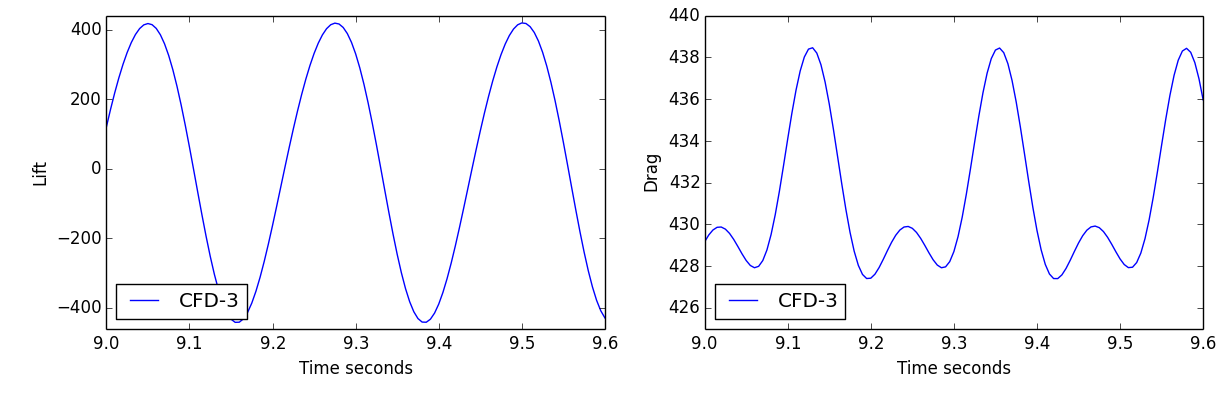
\includegraphics[scale=0.5]{./Fig/cfd3_liftdrag.png}
      \caption{CFD-3, lift and drag forces at time t = [9, 9.6].}
\end{figure}

\begin{figure}[h!]
  \centering
    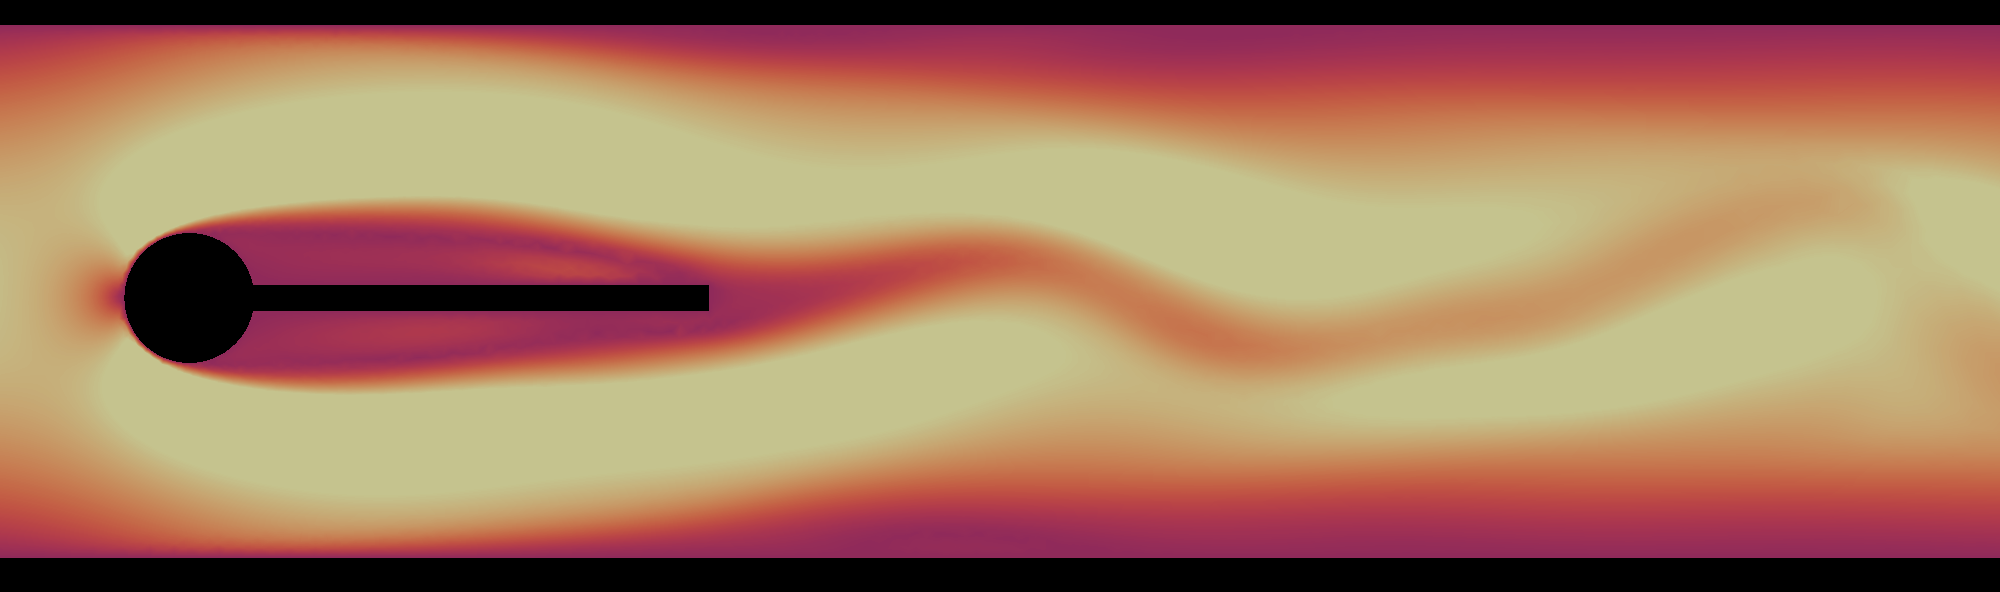
\includegraphics[scale=0.2]{./Fig/cfd3.png}
      \caption{CFD-3, flow visualization of velocity time t = 9s.}
\end{figure}

\newpage

\begin{table}[h!]
\centering
\label{CFD-3 Results}
\begin{tabular}{ |p{1cm}||p{2.9cm}|p{3.3cm}|p{3.3cm}|}
 \hline
  \multicolumn{4}{|c|}{$\Delta t = 0.01 \hspace{2mm} \theta = 0.5$} \\
   \hline
nel & ndof & Drag  & Lift \\
\hline
 1438    & 6881  (P2-P1)   & 417.23       +/-  0.0217 & -249.21       +/-  0.32  \\
   & 16474 (P3-P2)   & 414.86      $\pm$  5.6282 & -7.458      $\pm$  444.07  \\
 \hline
 2899    & 13648  (P2-P1) & 408.50  $\pm$   4.3029 & -19.731  $\pm$   373.45 \\  
     &  32853 (P3-P2)  & 432.86      $\pm$  5.5025 & -9.686      $\pm$  431.28  \\
  \hline
  7501    & 34657 (P2-P1) & 431.57  $\pm$   5.2627 & -12.497  $\pm$   429.76 \\    
    &  83955 (P3-P2)  & 438.20      $\pm$  5.5994 & -11.595      $\pm$  438.00 \\
    \hline
    19365   & 88520 (P2-P1) & 435.43  $\pm$   5.4133 & -11.545  $\pm$   438.89 \\
   &   215219 (P3-P2) & 438.80      $\pm$  5.6290 & -11.158      $\pm$  439.23 \\
\hline
 \multicolumn{2}{|c|}{Reference}  & 439.95 $\pm$ 5.6183 & -11.893 $\pm$ 437.81\\
 \hline
  \multicolumn{2}{|c|}{Error}  & 0.002 \% $\pm$ 0.001 \% & 0.061 \% $\pm$ 0.003\% \\
  \hline
  \end{tabular}
  \vspace{2cm}
 \begin{tabular}{ |p{1cm}||p{2.9cm}|p{3.3cm}|p{3.3cm}|}
  \hline
  \multicolumn{4}{|c|}{$\Delta t = 0.005 \hspace{2mm} \theta = 0.5$} \\
   \hline
nel & ndof & Drag  & Lift \\
\hline
 1438    & 6881  (P2-P1)   &  417.24  $\pm$  0.0084 & -249.386   $\pm$ 0.1345  \\
 1438    & 16474 (P3-P2)   & 414.90     $\pm$  5.7319 & -8.467 $\pm$  443.45  \\
\hline
 1438    &13648  (P2-P1)   & 408.27   $\pm$ 4.0192 & -18.981   $\pm$ 363.84 \\
 2899    &  32853 (P3-P2)   & 432.90      $\pm$  5.5333 & -11.382      $\pm$  430.60 \\
 \hline
 1438    & 34657  (P2-P1)   & 431.59 $\pm$5.2979 & -13.644   $\pm$ 429.68 \\
 7501    & 83955 (P3-P2)  & 438.23      $\pm$  5.6393 & -12.917 $\pm$  437.78 \\
 \hline
 1438    & 88520  (P2-P1)   & 435.46  $\pm$ 5.4579 & -13.190   $\pm$ 438.05 \\
 19365   & 215219 (P3-P2)  & 438.84    $\pm$  5.6576 & -12.786      $\pm$  438.36 \\
\hline
 \multicolumn{2}{|c|}{Reference}  & 439.95 $\pm$ 5.6183 & -11.893 $\pm$ 437.81\\
 \hline
  \multicolumn{2}{|c|}{Error}  & 0.002 \% $\pm$ 0.006 \% & 0.075 \% $\pm$ 0.001\% \\
  \hline
\end{tabular}
\caption{CFD-3 results, lift and drag evaluated at the inner geometry surface. A spatial refinement study is conducted for increasing mesh resolution and two different finite element pairs. The relative error is computed from the solution of the highest mesh resolution, against the reference solution.}
\label{table:cfd3}
\end{table}
\newpage

The numerical solutions of CFD-1 in Figure 4.2 shows convergence against the reference solution. Choosing P2-P1 elements together with a fully implicit scheme $\theta = 1$, a relative error of $0.006 \%$ for lift, and $0\%$ for drag is attained. For the numerical solution of CFD-2 presented in Figure 4.3, the same observations apply. The second order Crank–Nicolson scheme  $\theta = 0.5$ was investigated for CFD-1 and CFD-2, however only improving the results of order $10^{-6}$ for both lift and drag. For the periodic problem CFD-3, the choice of  P2-P1 elements with a fully implicit time-stepping scheme proved insufficient for capturing the expected periodic solution. Using Crank–Nicolson time-stepping scheme $\theta = 0.5$, the periodic solution was attained. 

\subsubsection*{Discussion}
Since the choice of finite-element pair is not reported in the original work, both P3-P2 and P2-P1 element pairs for fluid and pressure respectively was compared in combination with spatial mesh refinement. From Table 4.3, a relative error $ < 0.08\%$ of the mean and amplitude for lift and drag is attained. The choice P3-P2 element pair is eminent to achieve reasonable results for the first and second mesh regardless of time step.  However, the third and fourth mesh resolution shows close resemblance with the reference solution, independent of finite-element pair. On basis of the presented results, the fluid solver is validated in accordance with the proposed benchmark. 

\subsection{Validation of solid solver}
The validation of the solid solver is conducted on a rectangular domain, representing the elastic structure in Figure ~\ref{fig:tflag}.  The structure is fixed to a fictional wall on the left side of the domain, pulled by a gravitational force $\mathbf{g} = (0, g)$. The validation of the solid solver is based on comparison of the deflection of point $A(t) = [A_x(t), A_y(t)]$,  conducted on three refined mesh, where the number of finite elements are chosen in close resemblance with the original work in \cite{Hron2006}. A simple investigation of different finite-element pairs, suggest that P3-P3 elements where used for making the reference solution. In this study, lower order finite-element pair was included, comparing shorter simulation time with solution accuracy. While computational time is not a major concern for the solid solver, the study is important for potentially reducing the computational time for the final validation branch

\begin{table}[h!]
\centering.
\label{my-label}
\begin{tabular}{ |p{3cm}||p{2cm}|p{2cm}|p{2cm}|  }
 \hline
 parameter              & CSM 1 & CSM 2 & CSM 3 \\
 \hline
$\rho^s [10^{3}\frac{kg}{m^3}]$ & 1    & 1    & 1    \\
$\nu^s $  & 0.4    & 0.4    & 0.4    \\
$\mu^s  [10^{6}]$  & 0.5    & 2.0    & 0.5    \\
$g  \frac{m}{s^2}]$  & 2.0    & 2.0    & 2.0    \\
\hline
\end{tabular}
\caption{Solid sub-problem parameters}
\end{table}

\newpage

\subsubsection*{Results}
The numerical results for CSM-1, CSM-2, and CSM-3 are presented in table Table ~\ref{table:csm1}, ~\ref{table:csm2}, ~\ref{table:csm31}, and ~\ref{table:csm32}. For the steady state sub-problems CSM-1 and CSM-2, a spatial convergence study is conducted through mesh refinement with three different finite-element pairs. For the periodic CSM-3 problem, an additional temporal study was conducted for two different time steps. In Figure ~\ref{fig:bender}, a visualization of CSM-3 is provided for three different time steps. Finally, Figure ~\ref{fig:csm3c} shows the displacement vector components, comparing all finite-element pairs for the finest mesh resolution. \\

 For CSM-1, the relative error of deformation found in Table 4.6, is $1.41 \%$ and $0.8\%$ for the x and y coordinate respectively. In Table 4.7, a relative error of   $1.49 \%$ and $0.88\%$ for the x,y components can be found for CSM-2, proving both steady state problems coincide with the reference solution. In Table 4.8, the numerical solutions CSM-3 for time steps $\Delta t = 0.01$ and $\Delta t = 0.005$, are in close resemblance with the reference solution. The study of lower-order elements proved successful for all problems, justifying accurate results can be achieved using P2-P2 elements for deformation and velocity, even for coarse mesh resolution. 

\begin{table}[h!]
\centering
\begin{tabular}{ |p{1cm}||p{2.7cm}|p{3.3cm}|p{3.3cm}|}
\hline
  \multicolumn{4}{|c|}{$\Delta t = 0.1 \hspace{2mm} \theta = 1.0$} \\
\hline
nel & ndof & ux of A [x $10^{-3}$]  &uy of A [x $10^{-3}$] \\
\hline
 319     & 832 P1-P1  & -5.278 &  -56.6 \\
     & 2936 P2-P2 & -7.056 &  -65.4 \\
      & 6316 P3-P3 &  -7.064 &   -65.5  \\
 \hline
  1365    & 3140 P1-P1  & -6.385 &  -62.2 \\
     & 11736 P2-P2 & -7.075 &  -65.5 \\
     & 25792 P3-P3 & -7.083 &  -65.5 \\
 \hline
  5143    & 11084 P1-P1 & -6.905 &  -64.7  \\
     & 42736 P2-P2 & -7.083 &  -65.4\\
     & 94960 P3-P3 & -7.085 &  -65.5  \\
  \hline
  \multicolumn{2}{|c|}{Reference}  &-7.187    & -66.1 \\
   \hline
    \multicolumn{2}{|c|}{Error}  & 1.41 \%   & 0.8 \%\\
   \hline
\end{tabular}
\caption{CSM-1, deformation components of A(t) for $\Delta t = 0.1$ and increasing spatial refinement. The error is computed as the relative error from the highest mesh resolution against the reference solution.}
\label{table:csm1}
\end{table}

\begin{table}[h!]
\centering
\begin{tabular}{ |p{1cm}||p{2.7cm}|p{3.3cm}|p{3.3cm}|}
\hline
  \multicolumn{4}{|c|}{$\Delta t = 0.05 \hspace{2mm} \theta = 1.0$} \\
\hline
nel & ndof & ux of A [x $10^{-3}$]  &uy of A [x $10^{-3}$] \\
\hline

 319     & 832 P1-P1  & -0.3401 &  -14.43  \\ 
     & 2936 P2-P2 &  -0.460  &  -16.78  \\ 
      & 6316 P3-P3 & -0.461 &  -16.79  \\
        \hline
  1365    & 3140 P1-P1  &  -0.414 &  -15.93\\
     & 11736 P2-P2 &  -0.461 &  -16.81 \\
     & 25792 P3-P3 & -0.461  &  -16.82 \\
        \hline
   5143    & 11084 P1-P1 & -0.449 &  -16.60  \\
     & 42736 P2-P2 &-0.461 &  -16.82 \\
     & 94960 P3-P3 & -0.462 &  -16.82 \\
  \hline
  \multicolumn{2}{|c|}{Reference}  & -0.469      & -16.97  \\
   \hline
    \multicolumn{2}{|c|}{Error}  & 1.49\%   & 0.88 \%\\
   \hline
\end{tabular}
\caption{CSM-2, deformation components of A(t) for $\Delta t = 0.05$ and increasing spatial refinement. The error is computed as the relative error from the highest mesh resolution against the reference solution.}
\label{table:csm2}
\end{table}

\newpage

\begin{table}[h!]
\centering
\begin{tabular}{ |p{1cm}||p{2.7cm}|p{3.3cm}|p{3.3cm}|}
\hline
  \multicolumn{4}{|c|}{$\Delta t = 0.01 \hspace{2mm} \theta = 0.5$} \\
\hline
nel & ndof & ux of A [x $10^{-3}$]  &uy of A [x $10^{-3}$] \\
\hline
    319     & 832 P1-P1 & -10.835       +/-  10.836 & -55.197       +/-  56.845 \\
     & 2936 P2-P2 & -14.390       +/-  14.392 & -63.303       +/-  65.149 \\
      & 6316 P3-P3& -14.432       +/-  14.435 & -63.397       +/-  65.263 \\
    \hline
    1365    & 3140 P1-P1  & -13.053       +/-  13.054 & -60.367       +/-  62.241 \\
     & 11736 P2-P2  & -14.428       +/-  14.432 & -63.388       +/-  65.256 \\
     & 25792 P3-P3  & -14.444       +/-  14.446 & -63.432       +/-  65.287 \\
     \hline
     5143    & 11084 P1-P1 & -14.082       +/-  14.084 & -62.656       +/-  64.495 \\
     & 42736 P2-P2 & -14.444       +/-  14.447 & -63.435       +/-  65.288 \\
     & 94960 P3-P3& -14.449       +/-  14.452 & -63.449       +/-  65.296 \\
 \hline
  \multicolumn{2}{|c|}{Reference}  &-14.305 +- -14.305        & -63.607 +- 65.160    \\
   \hline
    \multicolumn{2}{|c|}{Error}  & 1\% $\pm$ 1\%   & 0.24\% $\pm$ 0.24\%\\
   \hline
\end{tabular}
\caption{CSM-3, deformation components of A(t) for $\Delta t = 0.01$, with increasing temporal refinement. The error is computed as the relative error from the highest mesh resolution.}
\label{table:csm31}
\end{table}

\begin{table}[h!]
\centering
\begin{tabular}{ |p{1cm}||p{2.7cm}|p{3.3cm}|p{3.3cm}|}
\hline
  \multicolumn{4}{|c|}{$\Delta t = 0.005 \hspace{2mm} \theta = 0.5$} \\
\hline
nel & ndof & ux of A [x $10^{-3}$]  &uy of A [x $10^{-3}$] \\
\hline
    319     & 832 P1-P1 & -10.846       +/-  10.848 & -56.049       +/-  56.053 \\
     & 2936 P2-P2  & -14.390       +/-  14.391 & -63.738       +/-  64.703 \\
      & 6316 P3-P3 & -14.429       +/-  14.430 & -63.833       +/-  64.810 \\
 \hline 
    1365    & 3140 P1-P1 & -13.057       +/-  13.057 & -60.813       +/-  61.826 \\
     & 11736 P2-P2& -14.426       +/-  14.427 & -63.827       +/-  64.801 \\
     & 25792 P3-P3 & -14.440       +/-  14.441 & -63.854       +/-  64.845 \\
 \hline
      5143    & 11084 P1-P1 & -14.091       +/-  14.091 & -63.195       +/-  63.981 \\
     & 42736 P2-P2 & -14.441       +/-  14.441 & -63.856       +/-  64.847 \\
     & 94960 P3-P3 & -14.446       +/-  14.446 & -63.865       +/-  64.860 \\
 \hline
  \multicolumn{2}{|c|}{Reference}  &-14.305 +- -14.305        & -63.607 +- 65.160    \\
   \hline
    \multicolumn{2}{|c|}{Error}  & 1\% $\pm$ 1\% &  0.4\% $\pm$ 0.4\%  \\
   \hline
\end{tabular}
\caption{CSM-3, deformation components of A(t) for $\Delta t = 0.005$, with increasing temporal refinement. The error is computed as the relative error from the highest mesh resolution.}
\label{table:csm32}
\end{table}

\newpage
\begin{figure}
    \centering
    \begin{subfigure}[b]{0.3\textwidth}
        
\includegraphics[width=\textwidth]{./Fig/csm3_1.png}
       \caption{$t = 0$}
        \label{fig:gull}
    \end{subfigure}
    ~ %add desired spacing between images, e. g. ~, \quad, \qquad, \hfill etc. 
      %(or a blank line to force the subfigure onto a new line)
    \begin{subfigure}[b]{0.3\textwidth}
        
\includegraphics[width=\textwidth]{./Fig/csm3_2.png}
               \caption{$t = 0.22$}
        \label{fig:tiger}
    \end{subfigure}
    ~ %add desired spacing between images, e. g. ~, \quad, \qquad, \hfill etc. 
    %(or a blank line to force the subfigure onto a new line)
    \begin{subfigure}[b]{0.3\textwidth}
        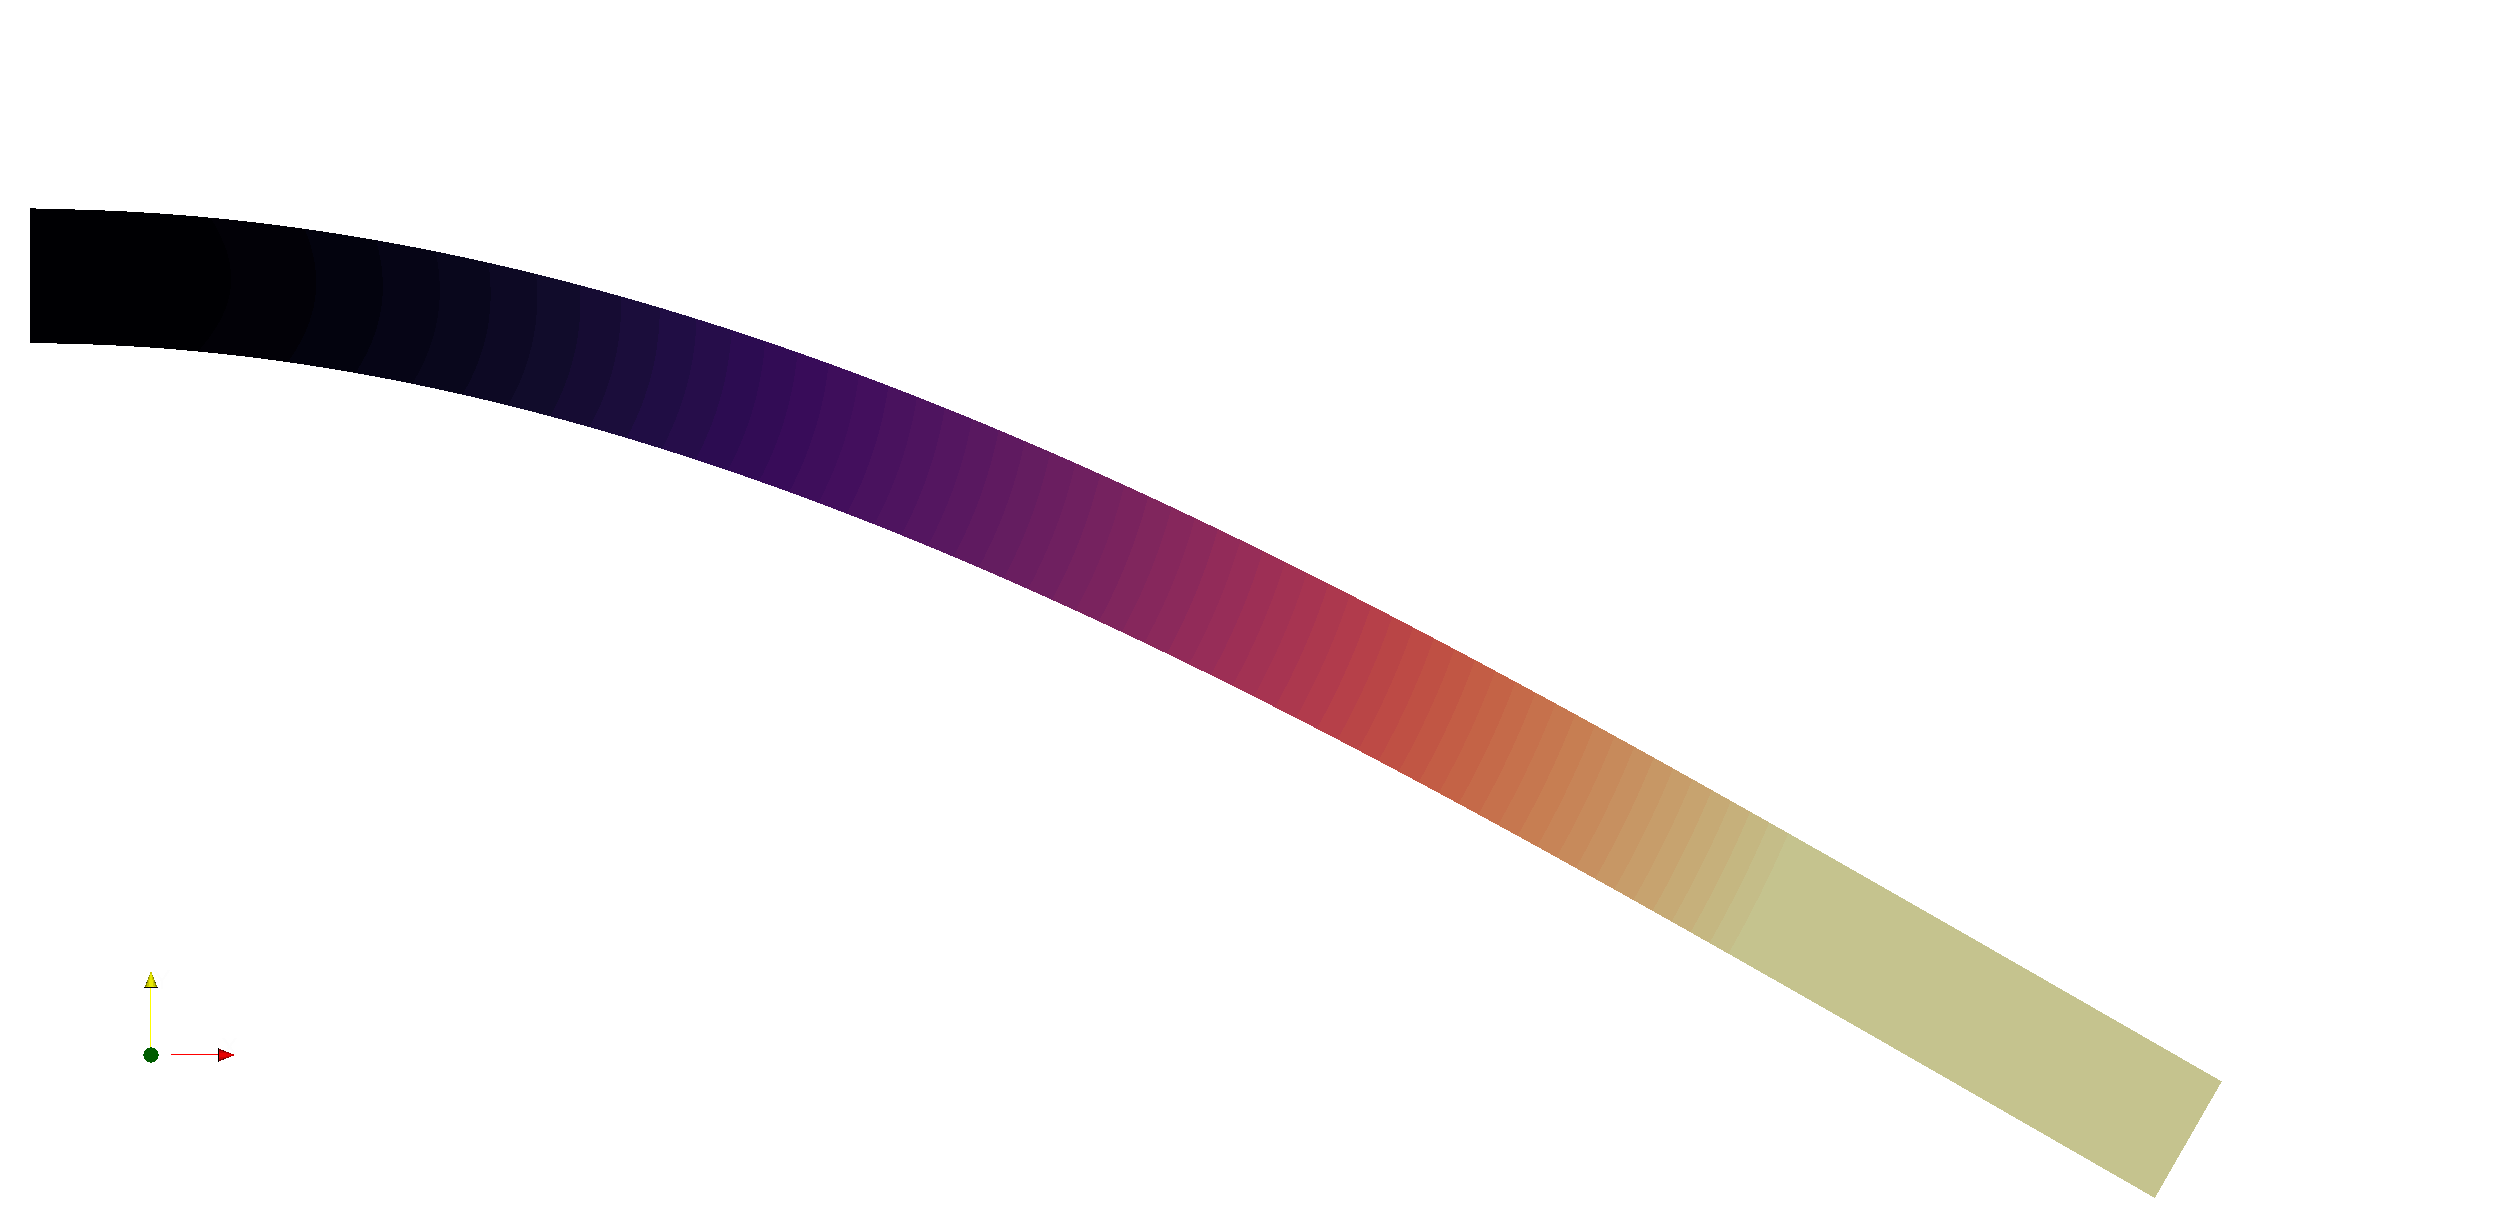
\includegraphics[width=\textwidth]{./Fig/csm3_3.png}
        \caption{$t = 0.45$}
        \label{fig:mouse}
    \end{subfigure}
    \caption{CSM-3, visualization of deformation of the elastic flag for three time steps: (a) initial configuration, (b) half way extenstion, (c) full extension }
 \label{fig:bender}
\end{figure}

\begin{figure}[h!]
  \centering
    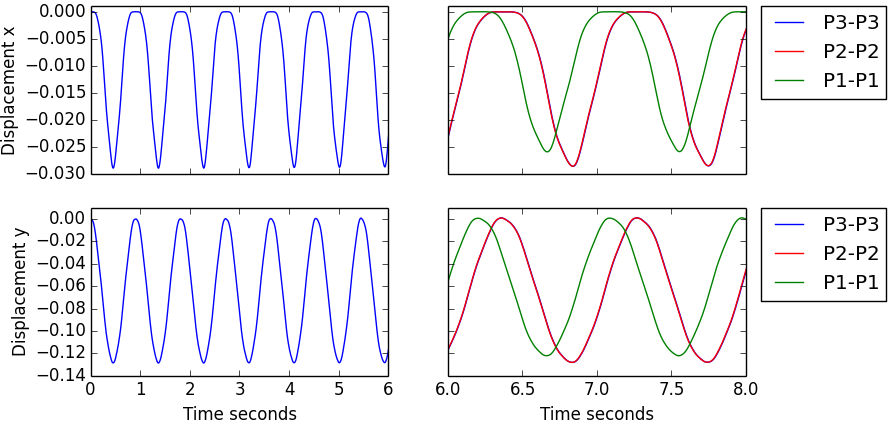
\includegraphics[scale=0.34]{./Fig/csm3compare.png}
      \caption{CSM-3 $\Delta t = 0.01$, deformation components of A(t) with finest mesh resolution, comparing all finite element pairs for time interval $t \in [0, 6]$  and $t \in [6, 8]$.}
       \label{fig:csm3c}
\end{figure}

\subsubsection*{Discussion}
 
 Comparing all finite-element pairs for CSM-3, visualized in figure 4.5, shows P2-P2 and P3-P3 elements hardly can be distinguished from each other. In accordance with previous mentioned results and observations, the solid solver is validated in accordance with the validation benchmark.
 

\subsection{Validation of fluid structure interaction solver}
\label{subsec:fsi3}
The validation of the FSI solver consist of three sub-problems which will be referred to FSI-1, FSI-2 and FSI-3. The FSI-1 problem yields a steady state solution for the system, inducing small deformations to the elastic flag. The FSI-2 and FSI-3 problems results in a periodic solution, where the elastic flag oscillates behind the cylinder. All sub-problems inherit the conditions from the previous validation branches, with the exception of no gravitational force on the elastic flag. On the fluid-structure interface $\Gamma$, we enforce the kinematic and dynamic boundary condition
\begin{align}
\mathbf{v}_f = \mathbf{v}_s \\
\mathbf{\sigma}_f \cdot \mathbf{n} = \mathbf{\sigma}_s \cdot \mathbf{n}
\end{align}
Apart from the accuracy of the reported values, the main purpose of the validation of the solver is twofold. First, it is of great importance to ensure that the overall coupling of the fluid-structure interaction problem is executed correctly. Second, a good choice of mesh extrapolation model is essential to avoid divergence of the numerical solution, due to mesh entanglement.  Based on experience in section, 4.2.1-2, the finite element pair P2-P1 for the fluid solver, and P2-P2 for the solid solver proved successful. Therefore the finite-elements P2-P2-P1 for deformation, velocity, and pressure are chosen for the numerical experiments. Higher order elements will not be examined, mainly due to long computational time, even for optimized solver approaches.

\newpage

\begin{table}[h!]
\centering
\label{my-label}
\begin{tabular}{ |p{3cm}||p{2cm}|p{2cm}|p{2cm}|  }
 \hline
 \multicolumn{4}{|c|}{Solid parameters} \\
 \hline
 parameter              & FSI-1 & FSI-2 & FSI-3 \\
 \hline
 $\rho^s [10^{3} \frac{kg}{m^3}]$ & 1    & 10   & 1    \\
$\nu^s$ & 0.4  & 0.4  & 0.4  \\
$\mu^s  [10^{6}\frac{kg}{ms^2}]$  & 0.5  & 0.5  & 2.0  \\
 \hline
 \multicolumn{4}{|c|}{Fluid parameters} \\
 \hline
$\rho^f [10^{3}\frac{kg}{m^3}]$ & 1    & 1    & 1    \\
$\nu^f  [10^{-3}\frac{m^2}{s}]$  & 1    & 1    & 1    \\
U                      & 0.2  & 1    & 2    \\
parameter              & FSI-1 & FSI-2 & FSI-3 \\
Re                     & 20   & 100  & 200 \\
\hline
\end{tabular}
\caption{Fluid-structure interaction sub-problem parameters}
\end{table}

\subsubsection*{Results}
The numerical results for FSI-1, FSI-2, and FSI-3  are shown in Table 4.10-12. For all sub-problems, a spatial convergence study has been conducted on three different meshes with increasing resolution, with the relative error of the finest spatial and temporal resolution. For FSI-1 in Table 4.10, an additional option is proposed, omitting mesh moving models from the monolithic variational form from section 3.2.2.  A comparison of the validation parameters lift, drag, and displacement with different mesh moving models can be found in Figure 4.2-3. Finally, Figure 4.7 and 4.9 visualize the flow field and deformation of the elastic flag for a given time.
 
 \newpage
\subsubsection{FSI-1}

\begin{table}[h!]
\centering
\label{FSI-1 Results}
\begin{tabular}{ |p{1cm}||p{1cm}|p{2.8cm}|p{2.8cm}|p{2.7cm}|p{2.7cm}|p{1.2cm}|}
 \hline
  \multicolumn{6}{|c|}{Laplace} \\
   \hline
nel & ndof & ux of A [x $10^{-3}$]  &uy of A [x $10^{-3}$]& Drag  & Lift \\
 \hline
 2474    & 21249  &       0.0226 &       0.8200 & 14.061 & 0.7542 \\
 7307    & 63365  &       0.0227 &       0.7760 & 14.111 & 0.7517 \\
 11556   & 99810  &       0.0226 &      0.8220 & 14.201 & 0.7609 \\
  \hline
 \multicolumn{2}{|c|}{Reference} &  0.0227      &       0.8209      & 14.295  & 0.7638   \\
 \hline
     \multicolumn{2}{|c|}{Error}  & $ < 10^{-6}$  \% &  $ <10^{-6}$  \% & 0.66 \% & 0.38 \% \\
   \hline
\end{tabular}
\begin{tabular}{ |p{1cm}||p{1cm}|p{2.8cm}|p{2.8cm}|p{2.7cm}|p{2.7cm}|p{1.2cm}|}
 \hline
  \multicolumn{6}{|c|}{Linear Elastic} \\
   \hline
nel & ndof & ux of A [x $10^{-3}$]  &uy of A [x $10^{-3}$]& Drag  & Lift \\
 \hline
 2474    & 21249  &       0.0226 &       0.8198 & 14.061 & 0.7541 \\
 7307    & 63365  &       0.0227 &       0.7762 & 14.111 & 0.751  \\
 11556   & 99810  &       0.0226  &       0.8222 & 14.201 & 0.7609 \\
  \hline
 \multicolumn{2}{|c|}{Reference} &  0.0227      &       0.8209      & 14.295  & 0.7638   \\
 \hline
    \multicolumn{2}{|c|}{Error}  &$ < 10^{-6}$  \% &  $ <10^{-6}$  \%  & 0.66 \% & 0.38 \% \\
 \hline
\end{tabular}
\begin{tabular}{ |p{1cm}||p{1cm}|p{2.8cm}|p{2.8cm}|p{2.7cm}|p{2.7cm}|p{1.2cm}|}
 \hline
  \multicolumn{6}{|c|}{Biharmonic bc1} \\
   \hline
nel & ndof & ux of A [x $10^{-3}$]  &uy of A [x $10^{-3}$]& Drag  & Lift \\
 \hline
 2474    & 21249  &       0.0226 &       0.8200 & 14.061 & 0.7541 \\
 7307    & 63365  &       0.0227  &       0.7761 & 14.111 & 0.7517 \\
 11556   & 99810  &       0.0227  &       0.8017 & 14.205 & 0.9248 \\
  \hline
 \multicolumn{2}{|c|}{Reference} &  0.0227      &       0.8209      & 14.295  & 0.7638   \\
 \hline
    \multicolumn{2}{|c|}{Error}  & $ < 10^{-6}$  \% &  $ <10^{-6}$  \%  & 0.63 \% & 21.08 \% \\
 \hline
\end{tabular}
\begin{tabular}{ |p{1cm}||p{1cm}|p{2.8cm}|p{2.8cm}|p{2.7cm}|p{2.7cm}|p{1.2cm}|}
 \hline
  \multicolumn{6}{|c|}{Biharmonic bc2} \\
   \hline
nel & ndof & ux of A [x $10^{-3}$]  &uy of A [x $10^{-3}$]& Drag  & Lift \\
 \hline
 2474    & 21249  &       0.0226 &       0.8200 & 14.061 & 0.7543 \\
 7307    & 63365  &       0.0227 &       0.7761 & 14.111 & 0.7518 \\
 11556   & 99810  &       0.0227 &       0.8020 & 14.205 & 0.9249  \\
  \hline
 \multicolumn{2}{|c|}{Reference} &  0.0227      &       0.8209      & 14.295  & 0.7638   \\
 \hline
    \multicolumn{2}{|c|}{Error}  & $ < 10^{-6}$  \% &  $ <10^{-6}$  \%  & 0.63 \% & 21.09 \% \\
 \hline
\end{tabular}

\begin{tabular}{ |p{1cm}||p{1cm}|p{2.8cm}|p{2.8cm}|p{2.7cm}|p{2.7cm}|p{1.2cm}|}
 \hline
  \multicolumn{6}{|c|}{No extrapolation} \\
   \hline
nel & ndof & ux of A [x $10^{-3}$]  &uy of A [x $10^{-3}$]& Drag  & Lift \\
 \hline
 2474    & 21249  &       0.0224 &       0.9008 & 14.064 & 0.7713 \\
 7307    & 63365  &       0.0226  &       0.8221 & 14.117 & 0.7660 \\
 11556   & 99810  &       0.0225 &       0.8787 & 14.212 & 0.7837 \\
   \hline
 \multicolumn{2}{|c|}{Reference} &  0.0227      &       0.8209      & 14.295  & 0.7638   \\
 \hline
    \multicolumn{2}{|c|}{Error}  &   $ < 10^{-6}$  \% &  $ <10^{-5}$  \% & 0.58 \% & 2.61 \%  \\
 \hline
\end{tabular}
\caption{FSI 1 - Comparison of mesh extrapolation models for three spatial refinements}
\end{table}

\newpage
\subsubsection{FSI-2}

\begin{table}[h!]
\centering
\label{my-label}
\begin{tabular}{ |p{1cm}||p{1cm}|p{3.2cm}|p{3.2cm}|p{2.9cm}|p{3.1cm}|p{1.2cm}|}
 \hline
  \multicolumn{6}{|c|}{Laplace \hspace{2mm} $\Delta t = 0.01$  \hspace{2mm}  $\theta = 0.51$} \\
   \hline
nel & ndof & ux of A [x $10^{-3}$]  &uy of A [x $10^{-3}$]& Drag  & Lift \\
 \hline
 2474    & 21249  & -15.27  $\pm$ 13.45 & 1.34  $\pm$  82.4 & 157.00  $\pm$14.85 & -1.09  $\pm$258.47 \\
 7307    & 63365  &   -14.23  $\pm$13.37 & 1.31   $\pm$ 82.2 & 159,3 $\pm$ 15.43 & 0.92$\pm$ 254.53  \\
 11556   & 99810  & -14.96 $\pm$ 13.24 & 1.28  $\pm$ 81.9 & 161.07 $\pm$  17.81 & 0.02  $\pm$ 256.04  \\
 \hline
  \multicolumn{6}{|c|}{$\Delta t = 0.001$  \hspace{2mm}  $\theta = 0.5$} \\
   \hline
 nel & ndof & ux of A [x $10^{-3}$]  &uy of A [x $10^{-3}$]& Drag  & Lift \\
    \hline
 2474    & 21249  & -15.61$\pm$  13.21 & 1.34  $\pm$ 83.6 & 155.38   $\pm$   13.98 & -3.00  $\pm$   289.06 \\
 7307    & 63365  & -15.31  $\pm$ 13.07 & 1.02    $\pm$  82.8 & 156.81  $\pm$  14.95 & -2.00   $\pm$   276.24 \\
 11556   & 99810  & -15.28   $\pm$  13.04 & 1.28 $\pm$ 82.9 & 158.45  $\pm$  16.09 & -2.53   $\pm$  276.13 \\
 \hline
  \multicolumn{2}{|c|}{Reference} & -14.58 $\pm$ 12.44   & 1.23 $\pm$80.6    & 208.83 $\pm$ 73.75 & 0.88 $\pm$ 234.2 \\
   \hline
    \multicolumn{2}{|c|}{Error}  & (4.8 $\pm$  4.8)$10^{-6}$ \% &  (4 $\pm$ 2.8) $10^{-6}$\% & 24.1 \% $\pm$ 78.1 \% & 387.5 \% $\pm$ 17.9 \%   \\
   \hline
\end{tabular}
\end{table}

\begin{table}[h!]
\centering
%\caption{FSI 2 - Biharmonic BC1}
\label{my-label}
\begin{tabular}{ |p{1cm}||p{1cm}|p{3.2cm}|p{3.2cm}|p{2.9cm}|p{3.1cm}|p{1.2cm}|}
 \hline
  \multicolumn{6}{|c|}{Biharmonic 1 \hspace{2mm} $\Delta t = 0.01$  \hspace{2mm}  $\theta = 0.51$} \\
   \hline
nel & ndof & ux of A [x $10^{-3}$]  &uy of A [x $10^{-3}$]& Drag  & Lift \\
 \hline
 2474    & 21249  & -15.44 $\pm$  13.24 & -1.38 $\pm$  82.3   & 157.67  $\pm$  15.02 & -0.89$\pm$ 258.87 \\
 7307    & 63365  & -15.04 $\pm$ 12.96  & 0.99  $\pm$ 81.9 & 159.83$\pm$  16.83 & 0.98 $\pm$  245.40  \\
 11556   & 99810  & -15.29$\pm$ 13.17   & 1.29 $\pm$ 82.5 &  161.69 $\pm$   18.73 & -1.86 $\pm$ 251.30 \\

 \hline
  \multicolumn{6}{|c|}{$\Delta t = 0.001$  \hspace{2mm}  $\theta = 0.5$} \\
   \hline
 nel & ndof & ux of A [x $10^{-3}$]  &uy of A [x $10^{-3}$]& Drag  & Lift \\
\hline
 2474    & 21249  & -15.36 $\pm$ 13.12 &  1.35 $\pm$ 83.1& 155.38   $\pm$   13.74 & -2.55 $\pm$ 285.19 \\ 
 7307    & 63365  & -15.23 $\pm$ 12.97 & 1.03$\pm$ 82.4 & 157.14  $\pm$  15.18 & -8.62   $\pm$  263.87 \\
 11556   & 99810  &-15.27 $\pm$ 12.99 & 1.31 $\pm$ 82.7 & 157.72  $\pm$ 15.58 & 3.34    $\pm$ 258.76  \\
 \hline
  \multicolumn{2}{|c|}{Reference} & -14.58 $\pm$ 12.44   & 1.23 $\pm$80.6    & 208.83 $\pm$ 73.75 & 0.88 $\pm$ 234.2 \\
 \hline
\multicolumn{2}{|c|}{Error}  & (4.7 $\pm$ 4.4)$10^{-6}$ \% & (6.5 $\pm$ 2.6)$10^{-6}$ \%  & 208.83 $\pm$ 73.75 & 0.88 $\pm$ 234.2 \\
 \hline
\end{tabular}
\end{table}

\begin{table}[h!]
\centering
%\caption{FSI 2 - Biharmonic BC2}
\label{my-label}
\begin{tabular}{ |p{1cm}||p{1cm}|p{3.2cm}|p{3.2cm}|p{2.9cm}|p{3.1cm}|p{1.2cm}|}
 \hline
  \multicolumn{6}{|c|}{Biharmonic 2 \hspace{2mm}  $\Delta t = 0.01$  \hspace{2mm}  $\theta = 0.51$} \\
   \hline
nel & ndof & ux of A [x $10^{-3}$]  &uy of A [x $10^{-3}$]& Drag  & Lift \\
 \hline
 2474    & 21249  & -14.93 $\pm$ 13.22 & 1.35 $\pm$ 81.5 & 157.76  $\pm$ 15.04 & -0.49  $\pm$  254.13 \\
 7307    & 63365  & -14.67$\pm$ 13.05 & 1.00$\pm$ 80.9& 159.59 $\pm$  16.77 & 2.22 $\pm$  248.11  \\
 11556   & 99810  & 1.58 $\pm$ 12.86 & 1.23$\pm$ 81.5& 161.85   $\pm$18.84 & -1.64  $\pm$  247.04 \\
 \hline
  \multicolumn{6}{|c|}{$\Delta t = 0.001$  \hspace{2mm}  $\theta = 0.5$} \\
   \hline
 nel & ndof & ux of A [x $10^{-3}$]  &uy of A [x $10^{-3}$]& Drag  & Lift \\
\hline
 2474    & 21249  & -15.63  $\pm$ 12.7 & 1.31 $\pm$ 82.9 & 155.55      $\pm$ 13.82 & -2.45   $\pm$ 281.18 \\
 7307    & 63365  &  -14,99 $\pm$ 12.81& 0.99$\pm$ 82.14& 156.86    $\pm$  15.05 & -1.65   $\pm$ 269.84 \\
 11556   & 99810  &  -15.26 $\pm$ 12.91 & 1.27  $\pm$ 81.8 & 156.86   $\pm$ 15.05 & -1.65 $\pm$ 269.84 \\
 \hline
\multicolumn{2}{|c|}{Reference} & -14.58 $\pm$ 12.44   & 1.23 $\pm$80.6    & 208.83 $\pm$ 73.75 & 0.88 $\pm$ 234.2 \\
 \hline
\multicolumn{2}{|c|}{Error}  & (4.6 $\pm$ 3.7)$10^{-6}$ \% & (3.2 $\pm$ 1.4)$10^{-6}$ \%& 24.8 \% $\pm$ 79.5 \% & 287.5 \% $\pm$ 15.2 \% \\
 \hline
\end{tabular}
\caption{FSI 1 - Comparison of mesh extrapolation models for $\Delta t = [0,01, 0,001]$, for three spatial refinements}
\end{table}

\newpage

\begin{figure}[h!]
  \centering
    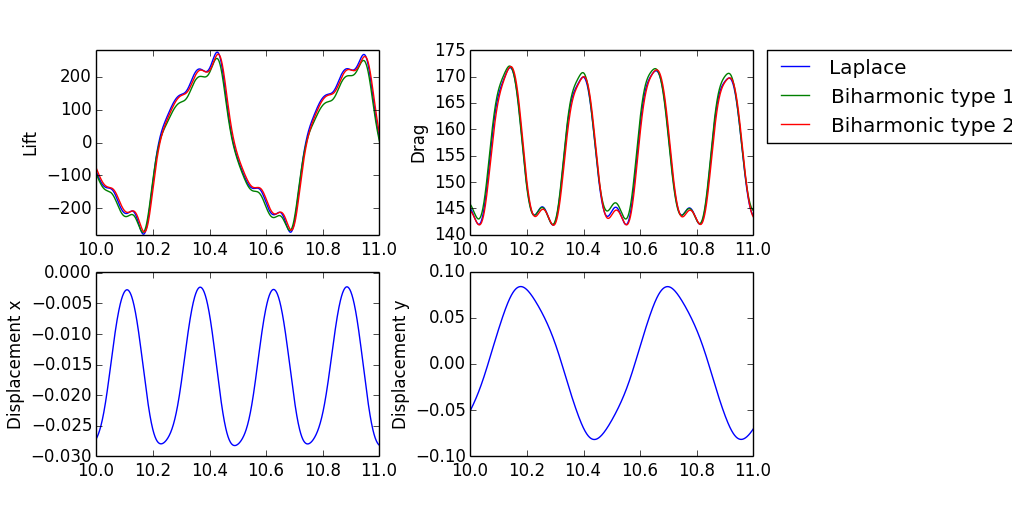
\includegraphics[scale=0.64]{./Fig/fsi2compare.png}
      \caption{FSI-2, visualization of fully developted flow with structure deformation at time t = 9s.}
\end{figure}

\begin{figure}[h!]
  \centering
    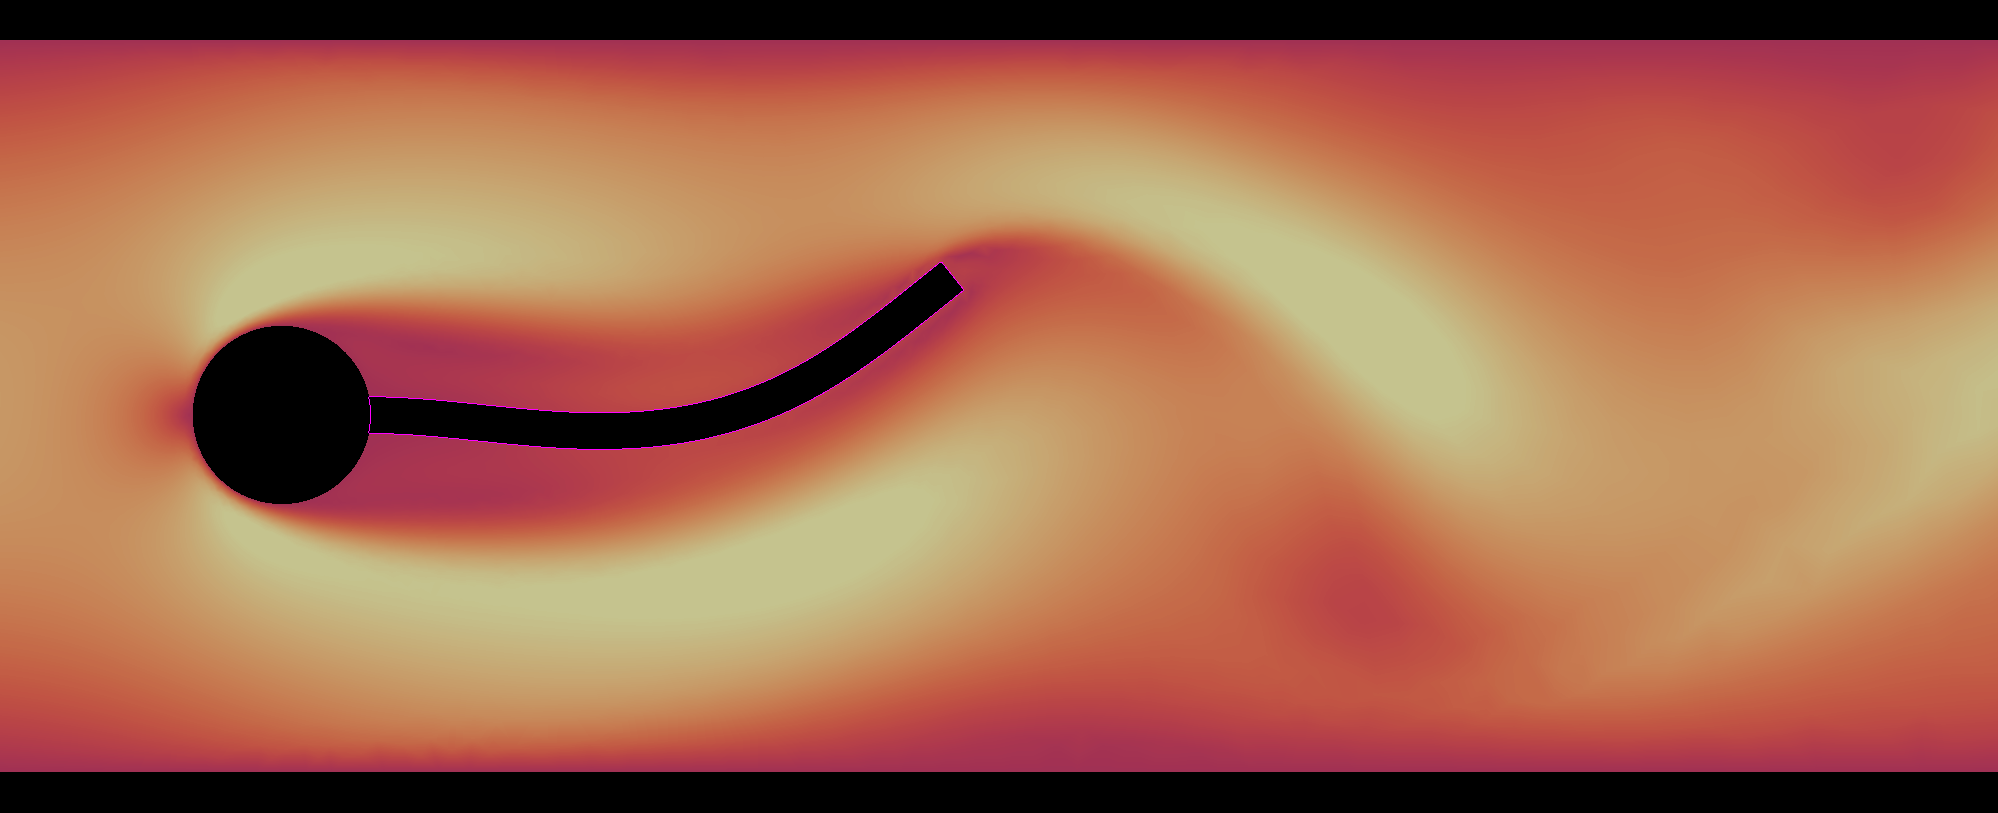
\includegraphics[scale=0.2]{./Fig/fsi2flow.png}
      \caption{FSI-2, visualization of fully developted flow with structure deformation at time t = 9s.}
\end{figure}

\newpage
\subsubsection{FSI-3}

\begin{table}[h!]
\centering
\caption{FSI 3 - Comparison of mesh extrapolation models}
\label{my-label}
\begin{tabular}{ |p{1cm}||p{1cm}|p{3.2cm}|p{3.2cm}|p{2.9cm}|p{3.1cm}|p{1.2cm}|}
 \hline
  \multicolumn{6}{|c|}{Laplace \hspace{2mm} $\Delta t = 0.01 \theta = 0.51$} \\
   \hline
nel & ndof & ux of A [x $10^{-3}$]  &uy of A [x $10^{-3}$]& Drag  & Lift \\
 \hline
 2474    & 21249  & -2.41 $\pm$   2.41 & 1.49     $\pm$   32.21 & 449.39       $\pm$   14.72 & 0.55 $\pm$   155.80  \\
 7307    & 63365  & -2.32    $\pm$   2.31 & 1.32 $\pm$    31.80 & 451.76  $\pm$   16.10 & 1.04      $\pm$   151.51  \\
 11556   & 99810  & -2.34  $\pm$   2.34  & 1.59   $\pm$  31.91 & 455.94       $\pm$ 17.34 & -0.01   $\pm$   151.36 \\
 \hline
  \multicolumn{6}{|c|}{$\Delta t = 0.001 \theta = 0.5$} \\
   \hline
 nel & ndof & ux of A [x $10^{-3}$]  &uy of A [x $10^{-3}$]& Drag  & Lift \\
    \hline
 2474    & 21249  & -2.91     $\pm$   2.74 & 1.28   $\pm$   35.01 & 450.90      $\pm$  18.11 & 2.28       $\pm$161.13 \\
 7307    & 63365  & -2.82    $\pm$   2.66& 1.24     $\pm$   34.69 & 453.56       $\pm$ 19.80 & 2.94     $\pm$ 158.67 \\
 11556   & 99810  & -2.88     $\pm$   2.72 & 1.49   $\pm$ 34.97 & 458.60   $\pm$ 22.12 & 2.23    $\pm$ 158.95 \\
 \hline
  \multicolumn{2}{|c|}{Reference} & -2.69 $\pm$  2.56                    & 1.48  $\pm$  34.38                   & 457.3  $\pm$  22.66        & 2.22  $\pm$ 149.78           \\
  \hline
    \multicolumn{2}{|c|}{Error}  & (7.0 $\pm$ 6.2)$10^{-6}$  \% & (6.7 $\pm$ 1.7)$10^{-6}$  \% & 0.28 \% $\pm$ 2.38 \% & 0.45 \% $\pm$ 6.12 \%\\
   \hline
\end{tabular}
\end{table}

\begin{table}[h!]
\centering
%\caption{FSI 3 - Biharmonic BC1}
\label{my-label}
\begin{tabular}{ |p{1cm}||p{1cm}|p{3.2cm}|p{3.2cm}|p{2.9cm}|p{3.1cm}|p{1.2cm}|}
 \hline
  \multicolumn{6}{|c|}{Biharmonic 1 \hspace{2mm}  $\Delta t = 0.01 \theta = 0.51$} \\
   \hline
nel & ndof & ux of A [x $10^{-3}$]  &uy of A [x $10^{-3}$]& Drag  & Lift \\
 \hline
 2474     &21249  & -2.40 $\pm$ 2.38  & 1.58 $\pm$ 32.07  & 450.16  $\pm$ 15.11  & -20.09 $\pm$ 148.17 \\
 7307    & 63365  &  -2.26 $\pm$ 2.14  & 1.70  $\pm$ 31.3 & 457.37  $\pm$ 15.24 & -51.77 $\pm$ 127.28 \\
 11556   & 99810  &   -2.33 $\pm$ 2.32 &  1.93   $\pm$ 31.5  & 456.40 $\pm$ 17.45 &  0.45 $\pm$ 149.68  \\
 \hline
  \multicolumn{6}{|c|}{$\Delta t = 0.001 \theta = 0.5$} \\
   \hline
 nel & ndof & ux of A [x $10^{-3}$]  &uy of A [x $10^{-3}$]& Drag  & Lift \\
 2474    & 21249  & -2.18 $\pm$ 2.10& 3.52 $\pm$ 2.90 & 435.19   $\pm$   9.77  & -1.59$\pm$   151.45 \\
 7307    & 63365  & -2.80 $\pm$ 2.64 & 1.25 $\pm$ 3.45 & 454.38   $\pm$   19.76 & 17.97  $\pm$  155.08 \\
 11556   & 99810  & -2.84 $\pm$ 2.68  & 1.50 $\pm$ 3.47 & 459.12    $\pm$   22.97 & -3.12     $\pm$ 171.22 \\
 \hline
 \multicolumn{2}{|c|}{Reference} & -2.69 $\pm$  2.56                    & 1.48  $\pm$  34.38                   & 457.3  $\pm$  22.66        & 2.22  $\pm$- 149.78           \\
 \hline
 \multicolumn{2}{|c|}{Error}  & (5.5 $\pm$ 4.6)$10^{-6}$ \% & (1.3 $\pm$ 8.9)$10^{-6}$ \%  & 0.40 \% $\pm$ 1.37 \% & 240.5 \% $\pm$ 14.3 \%\\
 \hline
\end{tabular}
\end{table}

\begin{table}[h!]
\centering
%\caption{FSI 3 - Biharmonic BC2}
\label{my-label}
\begin{tabular}{ |p{1cm}||p{1cm}|p{3.2cm}|p{3.2cm}|p{2.9cm}|p{3.1cm}|p{1.2cm}|}
 \hline
  \multicolumn{6}{|c|}{Biharmonic 2 \hspace{2mm}  $\Delta t = 0.01 \theta = 0.51$} \\
   \hline
nel & ndof & ux of A [x $10^{-3}$]  &uy of A [x $10^{-3}$]& Drag  & Lift \\
 \hline
 2474    & 21249  &-2.33 $\pm$ 2.33 & 1.57 $\pm$ 31.6    & 449.44  $\pm$ 14.82 & 0.80  $\pm$152.03  \\
 7307    & 63365  & -2.25 $\pm$ 2.23 &  1.35 $\pm$ 31.3  & 452.63     $\pm$16.29 & 17.11     $\pm$  146.05 \\
 11556   & 99810  & -2.25  $\pm$ 2.29 & 1.59  $\pm$ 31.4 & 457.89   $\pm$ 17.26 & 57.83      $\pm$  141.69 \\
 \hline
  \multicolumn{6}{|c|}{$\Delta t = 0.001 \theta = 0.5$} \\
   \hline
 nel & ndof & ux of A [x $10^{-3}$]  &uy of A [x $10^{-3}$]& Drag  & Lift \\
 2474    & 21249  & -2.83 $\pm$ 2.66   & 1.31 $\pm$ 34.5  &  450.24    $\pm$  18.25 & 2.57  $\pm$   175.42  \\
 7307    & 63365  & -2.77 $\pm$ 2.61    & 0.98$\pm$  34.6 & 453.53    $\pm$ 20.01 & 2.60   $\pm$ 159.13  \\
 11556   & 99810  & -2.80  $\pm$ 2.65 & 1.37 $\pm$ 34.7 & 458.41  $\pm$ 22.23 & 15.56   $\pm$  157.78 \\
 \hline
 \multicolumn{2}{|c|}{Reference} & -2.69 $\pm$  2.56                    & 1.48  $\pm$  34.38                   & 457.3  $\pm$  22.66        & 2.22  $\pm$- 149.78           \\
 \hline
 \multicolumn{2}{|c|}{Error}  & (4.0 $\pm$ 3.5)$10^{-6}$ \% & (7.4 $\pm$ 9.3)$10^{-6}$ \% & 0.24 \% $\pm$ 1.90 \% & 600.9 \% $\pm$ 5.34 \% \\
 \hline
\end{tabular}
\end{table}

\newpage

\begin{figure}[h!]
    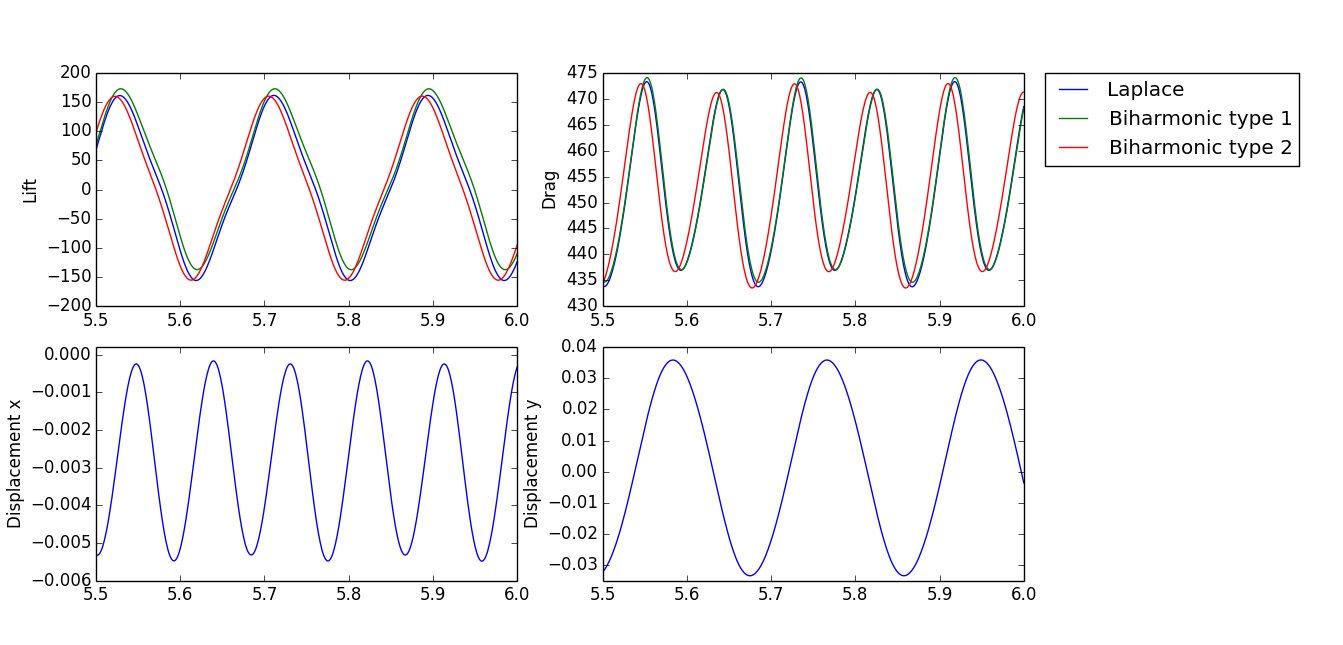
\includegraphics[scale=0.5]{./Fig/fsi3compare.png}
      \caption{Comparison of mesh motion models for FSI-3, in time interval t $t \in [5.5, 6]$.}
\end{figure}

\begin{figure}[h!]
  \centering
    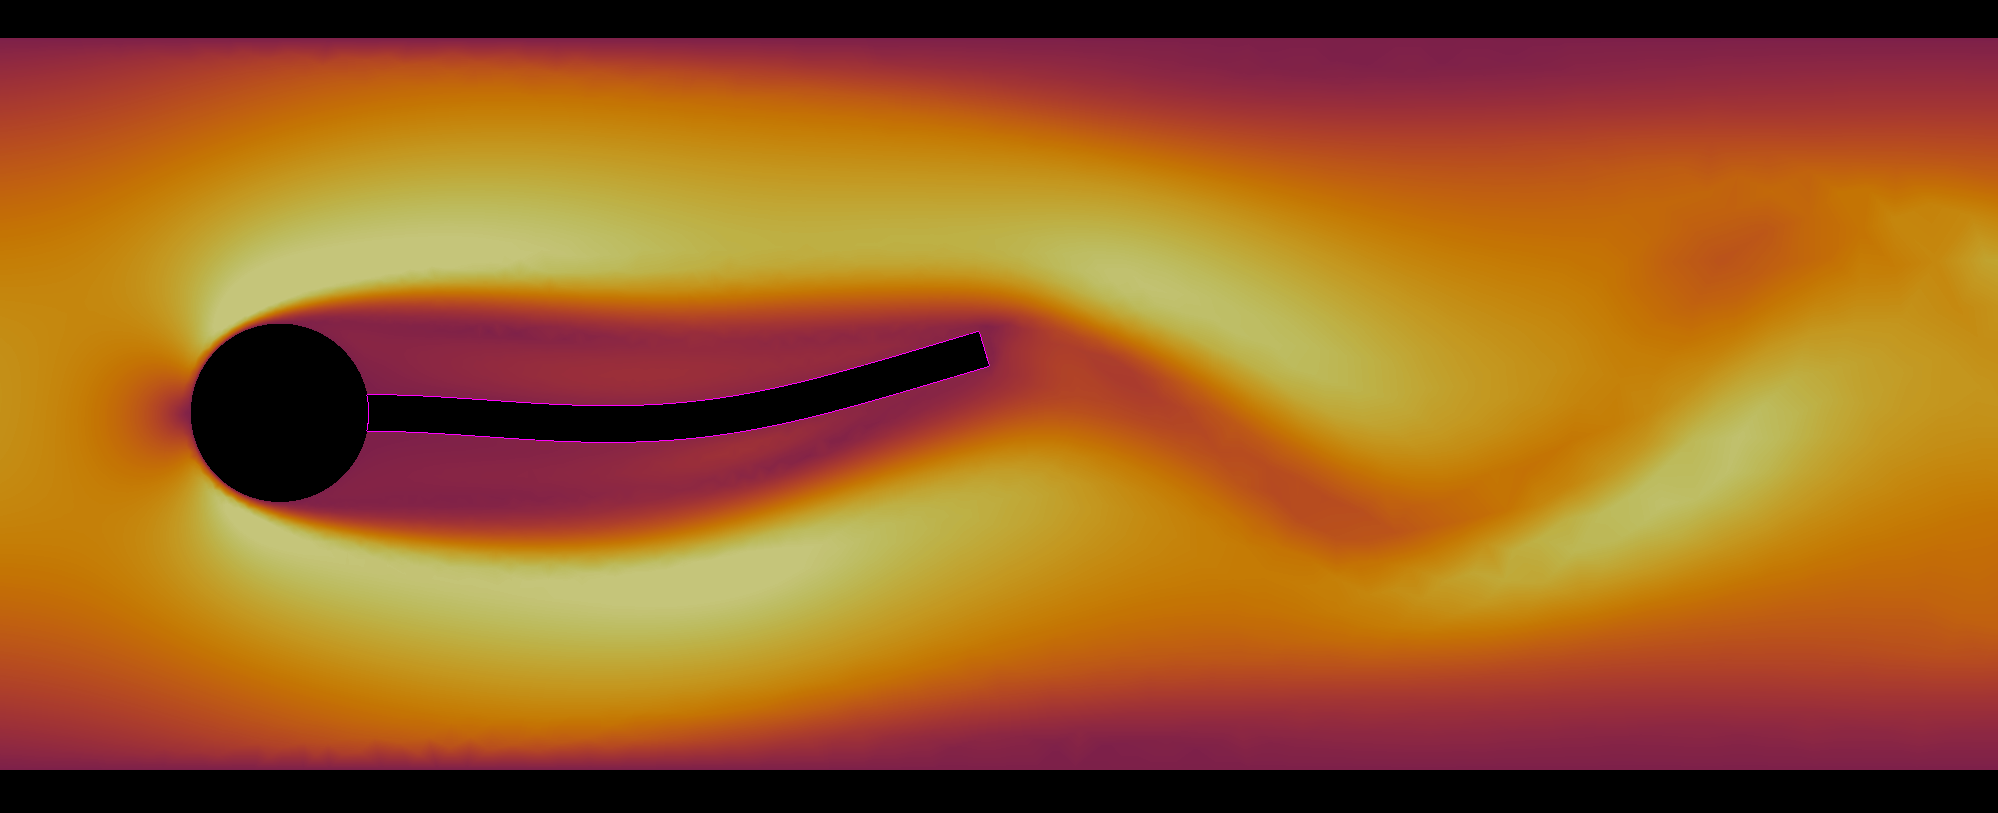
\includegraphics[scale=0.2]{./Fig/fsi3flow.png}
      \caption{FSI-3, visualization of fully developted flow with structure deformation at time t = 5.1s.}
\end{figure}

\newpage
\subsubsection*{Discussion}
For FSI-1, all models excel well in comparison with the reference solution, even at coarse mesh resolution. Due to low reynolds number flow the induced deformation of the elastic flag is very small, FSI-1 proves to be excellent for initial validation of fluid-structure interaction solvers. However, due the small deformations of the elastic flag of order $10^{-5}$,  FSI-1 doesn't provide a rigorous test case for mesh extrapolation models.  By omitting mesh extrapolation from the variatonal formulation in section 3.3.2,  reasonable results are still obtained in Table 4.10. This fact proves FSI-1 to be misleading in terms of mesh extrapolation model, but remains excellent for initial validation of fluid-structure interaction solvers and the overall coupling of the fluid and solid equations. \\

The FSI-2 problem proved to be one of the most demanding tests, due to the large deformation of the elastic flag. For large deformations, the chance of fluid mesh entanglement was considerably high, stressing the mesh moving models extensively. The linear elastic model failed for both time sizes, but not due to mesh entanglement but early failure of the Newton-solver. This finding is comparable with the investigation conducted in \cite{Richter2015}, where early failure of the Newton-solver is in context with long-term simulation of the implicit Crank-Nicolson scheme. In their study, a shifted implicit shifted Crank-Nicolson scheme $\theta = 0.5 + \Delta t$ proved to further improve stability for the newton-solver, making the numerical scheme stable for coarse time-step. Further, numerical investigation in \cite{Richter2015} showed that for both Crank-Nicolson and  shifted Crank-Nicolson are stable for $\Delta t < 0.003$ for the same benchmark. In my study, both implicit schemes was applicable for all mesh moving models, except the linear elastic model. \\

In general, the numerical solution regarding deformation of the elastic flag proved accurate in accordance with the reference solution for all sub-problems. However, the evaluation of drag and lift proved challenging for the periodic FSI-2 and FSI-3 problems. For FSI-2, poor accuracy was observed for all mesh resolutions and time steps, while for FSI-3 the evaluation of drag remained accurate. The same observations was found in \cite{Turek}, a followup work of the original benchmark \cite{Hron2006}, where numerical solutions committed by different research communities was compared. The diversity of lift and drag values provided by different research communities was surprising, as differences of order $50\%$ for drag and lift values, and $10\%$ for displacement was observed. More surprisingly was that the authors of the original benchmark \cite{Hron2006}, who also committed their numerical results, didn't match their own reference solution with the same solver. Therefore,  comparison of lift and drag forces with the reference solution alone can be misleading, and should not be the main acceptance criteria for code validation for this benchmark. Given the remarks in \cite{Turek}, the comparison of deformation is arguably a better main acceptance criteria. On this basis, the FSI code is validated in accordance with the original benchmark.  \\








 

%Validation of FSI is demanding due to the number of building blocks composing the full problem. For \textit{interface-tracking} methods such as the ALE-method, validation is not only related to the physical aspcets of the model. Even if the fluid and structure models excel well within predefined criteria, the non-physical nature of mesh moving models have proven to affect the numerical solution \cite{Wickb}. At first glance, this effect is surprising as mesh moving models simply describe the evolution of fluid mesh cells from the moving interface. However, each model distributes %t'he fluid cells differently, which in turn may have an important effect when conducting mathematical operations such %as gradients. 

\newpage
\chapter{Implementation of Fluid Structure Interaction}

For the general monolithic FSI problem, several complexities arise considering discretization. Yet divided, both the fluid and structure problem themselves impose rather difficult problems. These in combination with the coupling of the two sub-problems and their interaction to one another, makes even the most simplest implementation surprisingly difficult.  \\
Both problem 4.1, 4.2 introduces several non-linear contributions to the governing equations. Firstly the more familiar terms from the convection term of the fluid equation, and the stress tensor of the structure model. Second, the ALE method introduces an additional domain-velocity term to the advection in the fluid problem,  were spatial differential operators and time derivatives depending on other variables of interest. 
Nevn papers hvor investigations of term has been made.

\begin{prob}
\textit{ALE term}\begin{align*}
\ha{J} (\hat{F}_W^{-1}(\bat{v} - \pder{\ha{T}_W}{t}) \cdot \hat{\nabla}) \bat{v}
\end{align*}
\text{for the first type of boundary conditions introduced. } 
\end{prob}
The stability of the time-stepping have proven to be affected by the ALE advection term, which is difficult to control CITE(formaggia). This chapter will focus on the mentioned introduced problems by the monolithic ALE method. A brief description will be given for the most central components and technologies used for this thesis.   

\section{FEniCS}
The main component of this thesis is the FEniCS project, an open-source finite element environment for solving partial differential equations (https://fenicsproject.org/). Using a combination of high-level Python and C++ interfaces, mathematical models can be implemented compactly and efficiently. FEniCS consists of several sub-modules and we will give a brief overview of the most central components used during implementation and computation.

\subsection{DOLFIN}
DOLFIN is the computational C++ backend of the FEniCS project, and the main user interface. It unifies several FEniCs components for implementing of computational mesh, function spaces, functions and finite element assembly. 

\begin{itemize} 
\item UFL (The Unified Form Language)  is a domain specific language, used for the discretization of mathematical abstractions of partial differential equations on a finite element form. Its implementation on top of Python, makes it excellent to define problems close to their mathematical notation without the use of more complex features. One uses the term \textit{form} to define any representation of some mathematical problem defined by UFL.   

\item FFC (The form compiler) compiles the finite elements variation forms given by UFL, generating low-level efficient C++ code 

\item FIAT the finite element backend, covering a wide range of finite element basis functions used in the discretization of of the  the finite-element forms. It covers a wide range of finite element basis functions for lines, triangles and tetrahedras.

\end{itemize}  


DOLFIN also incorporate the necessary interfaces to external linear algebra solvers and data structures. Within FEniCS terminology these are called linear algebra backends. PETSc is the default setting in FEniCS, a powerful linear algebra library
with a wide range of parallel linear and nonlinear solvers and efficient as matrix and vector operations for applications written in C, C++, Fortran and Python.
\newpage

\section{Implementation}
As implementation of mathematics differ from the choices of programming languages and external libraries, a deep dive within the implementation in FEniCS will not be covered in this thesis. Only variational forms and solvers will be presented as to give the reader a general overview of the key concept and the interpretation of mathematics. Basic knowledge of coding is assumed of the reader. 

\subsection{Variational Form}
Implementation of the code-blocks of the fluid variational form given in Chapter 3, and Newton solver will be presented. It is not the intention to give the reader a deep review of the total implementation, but rather briefly point out key ideas intended for efficient speedup of the calculation. These ideas have proven essential as for the reduction of computation time of the complex problem.

\begin{python}[caption=thetaCN.py]
def F_(U):
	return Identity(len(U)) + grad(U)

def J_(U):
	return det(F_(U))

def sigma_f_u(u,d,mu_f):
    return  mu_f*(grad(u)*inv(F_(d)) + inv(F_(d)).T*grad(u).T)

def sigma_f_p(p, u):
    return -p*Identity(len(u))

def A_E(J, v, d, rho_f, mu_f, psi, dx_f):
    return rho_f*inner(J*grad(v)*inv(F_(d))*v, psi)*dx_f \
        + inner(J*sigma_f_u(v, d, mu_f)*inv(F_(d)).T, grad(psi))*dx_f


def fluid_setup(v_, p_, d_, n, psi, gamma, dx_f, ds, mu_f, rho_f, k, dt, v_deg, theta, **semimp_namespace):

	J_theta = theta*J_(d_["n"]) + (1 - theta)*J_(d_["n-1"])
	F_fluid_linear = rho_f/k*inner(J_theta*(v_["n"] - v_["n-1"]), psi)*dx_f

	F_fluid_nonlinear =  Constant(theta)*rho_f*inner(J_(d_["n"])*grad(v_["n"])*inv(F_(d_["n"]))*v_["n"], psi)*dx_f
	F_fluid_nonlinear += inner(J_(d_["n"])*sigma_f_p(p_["n"], d_["n"])*inv(F_(d_["n"])).T, grad(psi))*dx_f
	F_fluid_nonlinear += Constant(theta)*inner(J_(d_["n"])*sigma_f_u(v_["n"], d_["n"], mu_f)*inv(F_(d_["n"])).T, grad(psi))*dx_f
	F_fluid_nonlinear += Constant(1 - theta)*inner(J_(d_["n-1"])*sigma_f_u(v_["n-1"], d_["n-1"], mu_f)*inv(F_(d_["n-1"])).T, grad(psi))*dx_f
	F_fluid_nonlinear +=inner(div(J_(d_["n"])*inv(F_(d_["n"]))*v_["n"]), gamma)*dx_f
	F_fluid_nonlinear += Constant(1 - theta)*rho_f*inner(J_(d_["n-1"])*grad(v_["n-1"])*inv(F_(d_["n-1"]))*v_["n-1"], psi)*dx_f
	F_fluid_nonlinear -= rho_f*inner(J_(d_["n"])*grad(v_["n"])*inv(F_(d_["n"]))*((d_["n"]-d_["n-1"])/k), psi)*dx_f

	return dict(F_fluid_linear = F_fluid_linear, F_fluid_nonlinear = F_fluid_nonlinear)
\end{python}

Alorithm 1.1 presents the implementation of the fluid residue, used in the Newton iterations. Apart from the rather lengthy form of the fluid residual, the strength of Unified Form Language preserving the abstract formulation of the problem is clear. The overall representation of the problem is by now just a form, its a representation and does not yet define vectors or matrices.

\begin{python}[caption=newtonsolver.py]
def newtonsolver(F, J_nonlinear, A_pre, A, b, bcs, \
              dvp_, up_sol, dvp_res, rtol, atol, max_it, T, t, **monolithic):
    Iter      = 0
    residual   = 1
    rel_res    = residual
    lmbda = 1

    while rel_res > rtol and residual > atol and Iter < max_it:
        if Iter % 4  == 0:
            A = assemble(J_nonlinear, tensor=A, form_compiler_parameters = {"quadrature_degree": 4}) 
            A.axpy(1.0, A_pre, True)
            A.ident_zeros()

        b = assemble(-F, tensor=b)

        [bc.apply(A, b, dvp_["n"].vector()) for bc in bcs]
        up_sol.solve(A, dvp_res.vector(), b)
        dvp_["n"].vector().axpy(lmbda, dvp_res.vector())
        [bc.apply(dvp_["n"].vector()) for bc in bcs]
        rel_res = norm(dvp_res, 'l2')
        residual = b.norm('l2')
        if isnan(rel_res) or isnan(residual):
            print "type rel_res: ",type(rel_res)
            t = T*T

\end{python}
\section{Optimization of Newtonsolver}
As for any program, the procedure of optimization involves finding the bottleneck of the implementation. Within computational science, this involves finding the area of code which is the primary consumer of computer resources. \\
As for many other applications, within computational science one can often assume the consummation of resources follows the \textit{The Pareto principle}. Meaning that for different types of events, roughly 80\% of the effects come from 20\% of the causes. An analogy to computational sciences it that 80\% of the computational demanding operations comes from 20\% of the code. In our case, the bottleneck is the newtonsolver. The two main reasons for this is 

\begin{itemize}
\item \textbf{Jacobian assembly} \\
The construction of the Jacobian matrix for the total residue of the system, is the most time demanding operations within the whole computation. 
\item \textbf{Solver}. \\ 
As iterative solvers are limited for the solving of fluid-structure interaction problems, direct solvers was implemented for this thesis. As such, the operation of solving a linear problem at each iteration is computational demanding, leading to  less computational efficient operations. Mention order of iterations?
\end{itemize}

Facing these problems, several attempts was made to speed-up the implementation. The FEniCS project consist of several nonlinear solver backends, were fully user-customization option are available. However one main problem which we met was the fact that FEniCS assembles the matrix of the different variables over the whole mesh, even though the variable is only defined in one to the sub-domains of the system.In our case the pressure is only defined within the fluid domain, and therefore the matrix for the total residual consisted of several zero columns within the structure region. FEniCS provides a solution for such problems, but therefore we were forced to construct our own solver and not make use of the built-in nonlinear solvers. \\

The main effort of speed-up were explored around the Jacobian assembly, as this was within our control.  

Of the speed-ups methods explored in this thesis we will specify that some of them were \textit{consistent} while others were \textit{nonconsistent}. Consistent methods are methods that always will work, involving smarter use of properties regarding the linear system to be solved. The non-consistent method presented involves altering the equation to be solved by some simplification of the system. As these simplifications will alter the expected convergence of the solver, one must take account for additional Newton iterations against cheaper Jacobi assembly. Therefore one also risk breakdown of the solver as the Newton iterations may not converge.   


\section{Consistent methods}
\subsection{Jacobi buffering}
By inspection of the Jacobi matrix, some terms of the total residue is linear terms, and remain constant within each time step. By assembling these terms only in the first Newton iteration will save some assembly time for the additional iterations needed each time step. As consequence the convergence of the Newton method should be unaffected as we do not alter the system.  

\section{Non-consisten methods}    
\subsection{Reuse of Jacobian}
As the assembly of the Jacobian at each iteration is costly, one approach of reusing the Jacobian for the linear system was proposed. In other words, the LU-factorization of the system is reused until the Jacobi is re-assembled. This method greatly reduced the computational time for each time step. By a user defined parameter, the number of iterations before a new assembly of the Jacobian matrix can be controlled. 

\subsection{Quadrature reduce}
The assemble time of the Jacobian greatly depends on the degree of polynomials used in the discretisation of the total residual. Within FEniCS this parameter can be controlled, and as such we can specify the order of polynomials representing the Jacobian. The use of lower order polynomials reduces assemble time of the matrix at each newton-iteration, however it leads to an inexact Jacobian which may results to additional iterations. 


 




  
\newpage


 \chapter{Numerical Experiments}

\section{Comparison of mesh moving models}
Mesh moving models are essential for numerical stability of fluid-structure interaction solvers. If the fluid mesh doesn't conform with the solid deformation, the risk of mesh entanglement increases with the possibility of instabilities or breakdown of the solver. In general, mesh models have shown to be either robust concerning mesh entanglements at the cost of computational time, or computational efficient with less robustness \cite{MM2016}. However, computational efficiency has proven not only to be dependent of the complexity of model, but also the regularity of the fluid mesh, reducing Newton iterations needed per time step \cite{Wickb}. \\ In this section we compare the mesh moving models from section 3.1.4. for the FSI-3 benchmark. The linear elastic model was found not applicable in section 4.2.3. Therefore, only the llaplace and biharmonic model will be considered. We will compare vertical displacement of the elastic flag, regularity of the fluid mesh, and number of Newton iterations per time step. To evaluate the regularity of the fluid mesh, the minimum value of the jacobian of the deformation gradient have been considered in \cite{Wickb}. 

\begin{align*}
{J}_f = det(\bat{F}_f) =  det(I + \hat{\nabla} \bat{u}_f)
\end{align*}
where $I$ is the identity matrix and $ \bat{u}_f$ is the fluid mesh deformation. The jacobian serves as a measure of mesh entanglement, meaning if $J_f \geq 0$, there are no crossing cells in the fluid mesh.  A serial naive Newton solver is used, avoiding any effects of speed-up techniques which may effect Newton iterations (see section 6.3.3). 

\newpage
\begin{figure}[h!]
 	\centering
    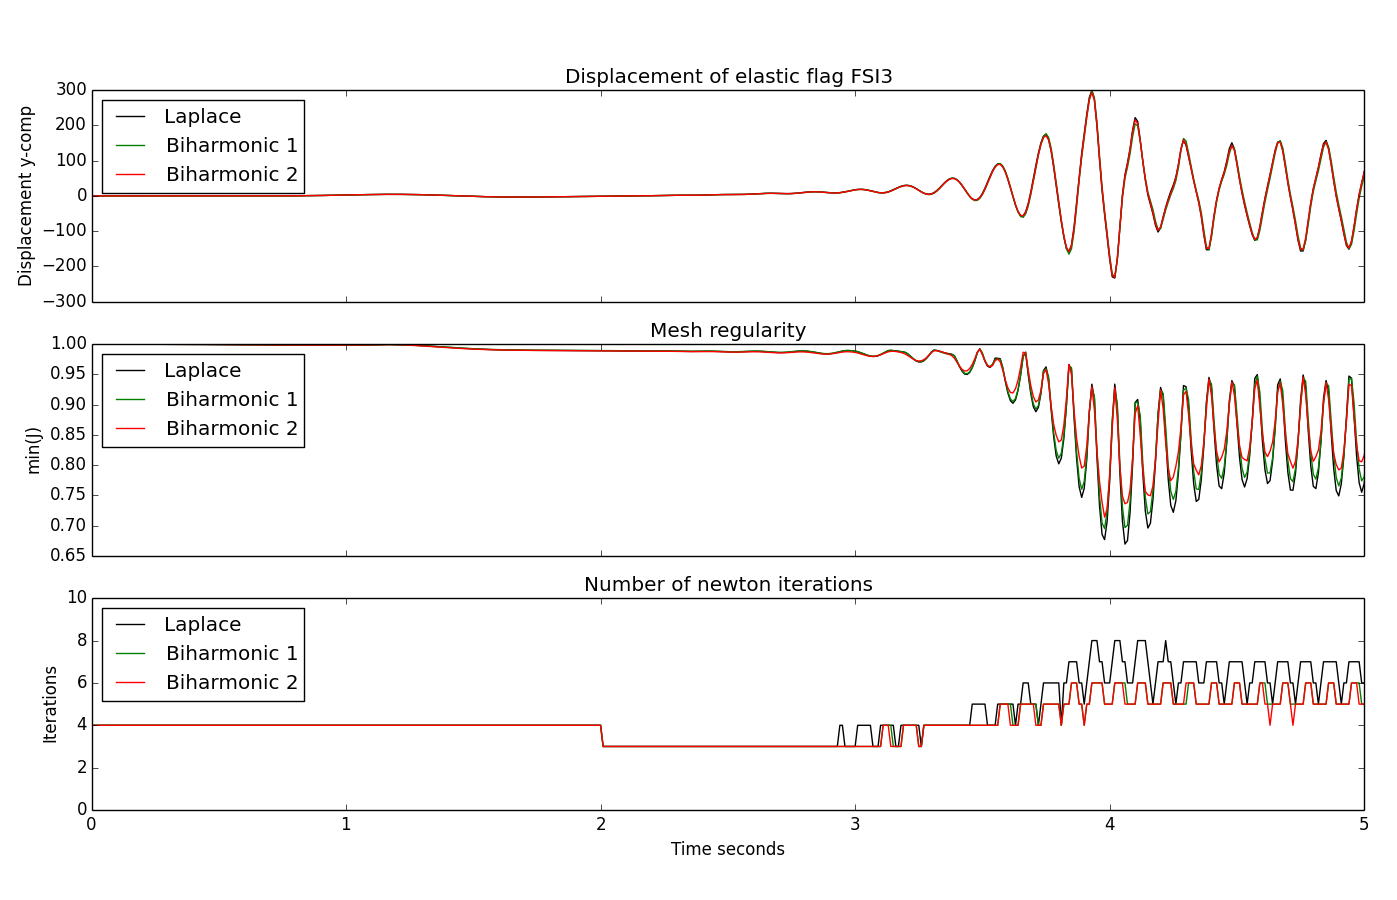
\includegraphics[scale=0.4]{./Fig/minjcompare.png} \\
      \caption{Investigation of mesh moving models for the FSI3 benchbark in the time interval $t \in [0, 5]$, comparing number of Newton iterations, mesh regularity, and vertical displacement of elastic flag. }
      \label{fig:minjcomp}
\end{figure}

\subsection*{Results}
Figure \ref{fig:minjcomp} compares the mesh moving models in the time interval  $t = [0, 5]$, when a stable periodic solution is obtained. All models shows a minima of mesh regularity at $3.8s < t < 4.2$, which is expected due to the largest deformation of the elastic flag. Both models shows a larger number of Newton-iterations are needed at each time step, when the elastic flag starts oscillating for $t > 3s$. The biharmonic models is superior in terms of number of iterations need per time step, and mesh regularity in comparison with the Laplace model. Further, the biharmonic 2 model shows better mesh regularity than biharmonic 1, but shows equal behavior in terms of Newton-iterations. For all models, no distinct difference in deformation of the y-component is found.

\subsection*{Discussion}
The numerical results confirms biharmonic models produce a better regularity of the fluid mesh cells, which in turn reduces the number of Newton-iterations needed per time step. However,  better evolution of mesh cells is by no means necessary for solving the FSI-3 problem. Therefore, the Laplace model remains a good choice, and its simplicity is preferable in terms of computational time (a topic to be discussed in section ~\ref{fig:cncomp1}). 
~\ref{sec:opti} 


\newpage

\section{Investigation of temporal stability}
One of the main challenges for constructing time-stepping schemes for ALE-methods, is the additional non-linearity introduced by the domain-velocity term in the fluid problem \cite{Formaggia2004}, 

\begin{align}
\ha{J}_f (\hat{F}_f^{-1}(\bat{v}_f - \pder{\ha{T}_f}{t}) \cdot \hat{\nabla}) \bat{v}_f
\end{align} 
Closer inspection of the convection term reviles spatial and temporal differential operators depending non-linearly on one another. These differential operators often appear separated, making discretization of a general time-stepping scheme not directly intuitive. The domain-velocity $ \pder{\ha{T}_f}{t}$ have proven to effect the stability of first and second-order time stepping schemes on fixed grids, but to what extent remains unclear  \cite{Formaggia2004, Formaggia1991}. The second order Crank-Nicolson used in this thesis, have also shown to suffer from temporal stability for long-term simulations of fluid problems, on fixed-grids \cite{Wick2013a}.
The  unconditionally stable Crank-Nicolson scheme is restricted by the condition \cite{Wick2013a},
\begin{align}
k \leq ch^{\frac{2}{3}} 
\end{align}
\textit{Where c is a costant, while k and h is the time-step and a mesh-size parameter } \\

while for the stability of the time derivative of the ALE-mapping, no accurate restriction is obtained (but thorough explored in \cite{Formaggia2004}). As a result, time step restriction is necessary to ensure that numerical stability  \cite{Formaggia2004}.  \\

The temporal stability for the implicit Crank-Nicolson scheme, for the validation benchmark chosen in this thesis, was studied in  \cite{Richter2015}. The criteria for the numerical experiments was to obtain a stable solution in the time interval of 10 seconds, by temporal and spatial refinement studies.  Following the ideas of \cite{Richter2015}, a second order scheme based on the Crank-Nicolson yields two possibilities.

\begin{discr}
\textit{Crank–Nicolson secant method }
\begin{align*}
\Big[\frac{\ha{J}(\bat{u}^{n}) \bat{\nabla} \bat{v}^{n} \bat{F}_W^{-1}}{2} 
+ \frac{\ha{J}(\bat{u}^{n-1}) \bat{\nabla} \bat{}v^{n-1} \bat{F}_W^{-1}}{2} \Big] 
\frac{\bat{u}^{n} - \bat{u}^{n-1}}{k}
\end{align*} 
\label{eq:cn1}
\end{discr}

\begin{discr}
\textit{Crank–Nicolson midpoint-tangent method}
\begin{align*}
\Big[\frac{\ha{J}(\bat{u}_{cn}) \bat{\nabla} \bat{v}_{cn} \bat{F}_W^{-1}}{2} \Big] 
\frac{\bat{u}^{n} - \bat{u}^{n-1}}{k} \hspace{4mm}
\bat{u}_{cn} = \frac{\bat{u}^{n} + \bat{u}^{n-1}}{2} \hspace{2mm}
\bat{v}_{cn} = \frac{\bat{v}^{n} + \bat{v}^{n-1}}{2}
\end{align*} 
\label{eq:cn2}
\end{discr}

\newpage

The numerical experiments showed very similar performance for Discretization  ~\ref{eq:cn1} and ~\ref{eq:cn2} , and significant differences of temporal accuracy was not found \cite{Richter2015}. However, spatial and temporal refinement showed the implicit Crank-Nicolson scheme gave stability problems for certain time-steps \textit{k}. Choosing $k = [0.005, 0.003]$, the FSI-3 problem (Section  ~\ref{subsec:fsi3}) suffered from numerical instabilities. Interestingly, the instabilities occurred earlier in simulation time for increasing mesh refinement. A similar experiment in  \cite{Wicka}, showed reducing the time step $k = 0.001$  yield stable long-time simulation for both  Discretization  ~\ref{eq:cn1} and ~\ref{eq:cn2}    \\

To coupe with the numerical unstabilities two approaches have been suggested in the litterature,  the \textit{shifted Crank-Nicolson}  and the \textit{frac-step method}  \cite{Richter2015, Wicka, Wick2013a},.  In this thesis the shifted Crank-Nicolson scheme was considered, introducing stability to the overall system by shifting the $\theta$ parameter slightly to the implicit side. If the shift is dependent of the time-step \textit{k} such that $\frac{1}{2} \leq \theta \leq \frac{1}{2} + k$, the scheme will be of second order \cite{Richter2015}. \\

\subsection{Results}
A numerical investigation of temporal stability in shown in Figure ~\ref{fig:cncomp1}, ~\ref{fig:cncomp2}, where the shifted Crank-Nicolson scheme $\theta = 0.5 + \Delta t$, is compared the original Crank-Nicolson $\theta = 0.5$. The shifted version clearly show stability properties surpassing the original Crank-Nicolson  scheme, for all numerical experiments. Choosing $\Delta t = 0.01$, the shifted Crank-Nicholson scheme retain long-time temporal stability, while capturing the physics of the benchmark. While for the ordinary Crank-Nicholson scheme, numerical experiments showed choosing $\Delta t = 0.001$ was necessarily to ensure stability, confirming the results found in \cite{Wicka}. Thus, reducing the time steps needed by a factor of ten. \\

Figure ~\ref{fig:cncomp1} shows choosing $\Delta t \in [0.2, 0.1]$ results in a steady-state solution.I believe this observation can be explained by influence the solid problem (Section \label{sec:solprob}). A centered Crank-Nicolson scheme $\theta= \frac{1}{2}$ is energy conservative, meaning little or no energy is dissipated. While a backward-Euler scheme $\theta = 1$  has little or no conservation of energy, meaning energy is easily dissipated from the system. The shifted Crank-Nicolson scheme dissipate more energy from the structure, if the choice of time step is sufficiently high, such as $\Delta t \in [0.2, 0.1] \rightarrow \theta = [0.7, 0.6]$.  Therefore, no periodic oscillation of the elastic flag is obtained. The validation of the solid solver shows this property, for the sub-problems CSM-1 and CSM-3. Given the same solid parameters, a steady-state solution is obtained for CSM-1 ($\theta = 1.0 $), while CSM-3 yields a periodic solution CSM-3 ($\theta = 0.5$ ), shown in Figure ~\ref{fig:csm1scm3} .\\

For  $\Delta t \in [0.05, 0.02]$,  the numerical scheme is close to centered, and conservation of energy is nearly preserved. However, spatial refinement by keeping a constant mesh resolution, initiates breakdown of the Newton-solver at an earlier time step. The breakdown is not due to mesh entanglement of the ALE-mapping, but divergence of Newton method \cite{Richter2015}. It is assumed that the divergence is linked to the influence of the domain velocity, by the research found in \cite{Formaggia2004}, but no clear time step restriction is obvious. Indeed, several works indicates choosing time step for a shifted Crank-Nicolson scheme is based on trial and error \cite{Wicka, Wick2013a}. 

\begin{figure}[h!]
 	\centering
    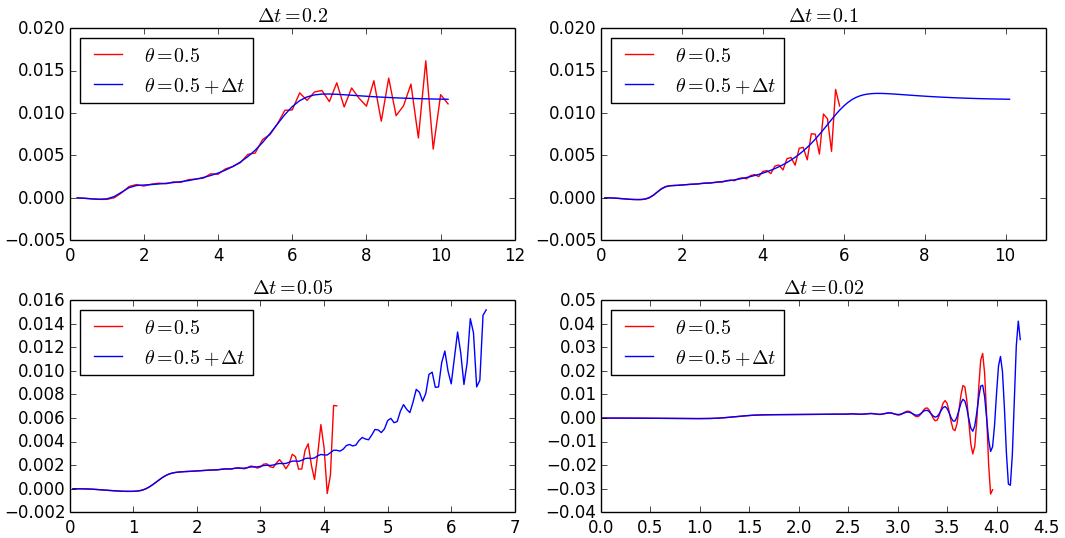
\includegraphics[scale=0.6]{./Fig/thetacheck.png} \\
      \caption{Investigation of temporal stability for the FSI3 benchbark in the time interval $t \in [0, 10]$, comparing the shifted and centered Crank-Nicolson scheme. }
\label{fig:cncomp1}
\end{figure}

\begin{figure}[h!]
 	\centering
    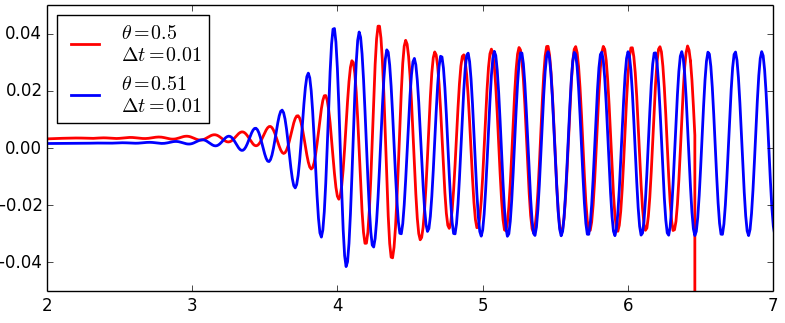
\includegraphics[scale=0.6]{./Fig/besttheta.png}
      \caption{Investigation of temporal stability for the FSI3 benchbark in the time interval $t \in [0, 10]$,  comparing the shifted and centered Crank-Nicolson scheme. }
\label{fig:cncomp2}
\end{figure}

\newpage

\begin{figure}[h!]
 	\centering
    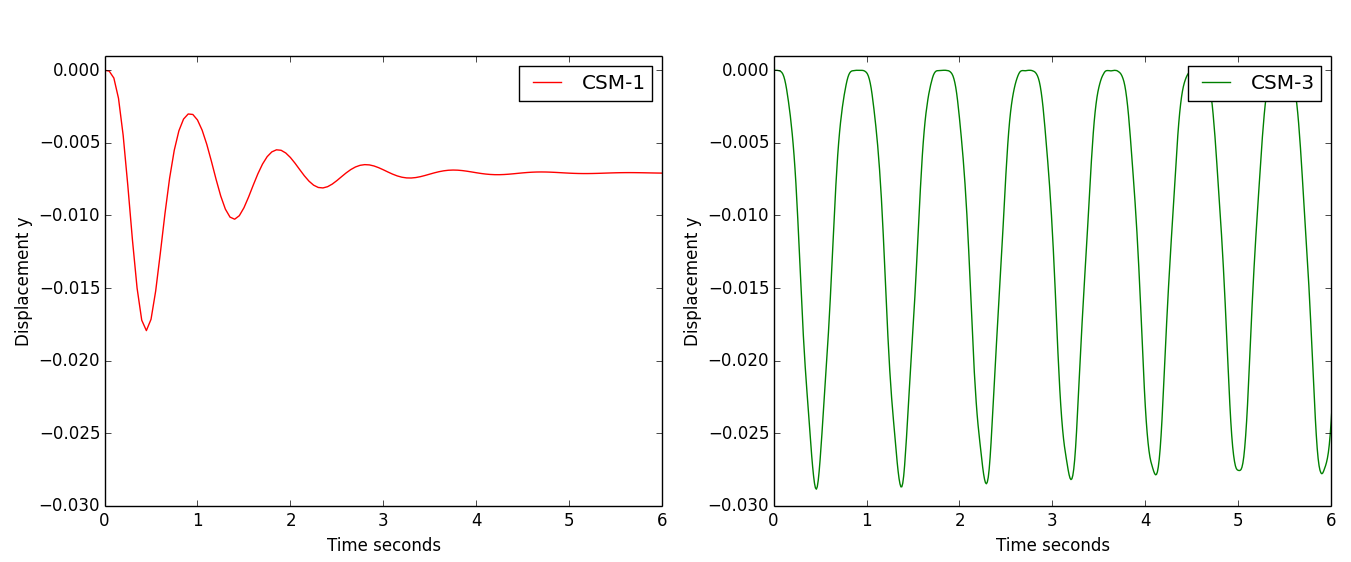
\includegraphics[scale=0.4]{./Fig/thetacompare.png}
      \caption{A comparison of a centered Crank-Nicolson scheme and backward Euler scheme}
\label{fig:csm1scm3}
\end{figure}


\newpage
\section{Optimization of the Newtonsolver}
\label{sec:opti}
A \textit{bottleneck} express a phenomena where the total performance of a complete implementation is limited to small code fragments, accounting for the primary consumption of computer resources.

As for many other applications, within computational science one can often assume the consummation of resources follows the \textit{The Pareto principle}. Meaning that for different types of events, roughly 80\% of the effects come from 20\% of the causes. An analogy to computational sciences it that 80\% of the computational demanding operations comes from 20\% of the code. In our case, the bottleneck is the newtonsolver. The two main reasons for this is 

\begin{itemize}
\item \textbf{Jacobian assembly} \\
The construction of the Jacobian matrix for the total residue of the system, is the most time demanding operations within the whole computation. 
\item \textbf{Solver}. \\ 
As iterative solvers are limited for the solving of fluid-structure interaction problems, direct solvers was implemented for this thesis. As such, the operation of solving a linear problem at each iteration is computational demanding, leading to  less computational efficient operations. Mention order of iterations?
\end{itemize}

Facing these problems, several attempts was made to speed-up the implementation. The FEniCS project consist of several nonlinear solver backends, were fully user-customization option are available. However one main problem which we met was the fact that FEniCS assembles the matrix of the different variables over the whole mesh, even though the variable is only defined in one to the sub-domains of the system.In our case the pressure is only defined within the fluid domain, and therefore the matrix for the total residual consisted of several zero columns within the structure region. FEniCS provides a solution for such problems, but therefore we were forced to construct our own solver and not make use of the built-in nonlinear solvers. \\

Newtons method can be written as,
\begin{align*}
\mathbf{F}(\mathbf{x}_n) + \nabla \mathbf{F}(\mathbf{x}_n)(\mathbf{x}_n - \mathbf{x}_0) = 0
\label{eq:newton}
\end{align*}
\textit{where $\mathbf{F}$ is the residue, $\mathbf{x}_n$, $\mathbf{x}_0$ is vector, and $ \nabla \mathbf{F}$ is the Jacobian of the residue} \\

Assembly of the Jacobian at each iteration is CPU-intensive, hence the main speed-up effort were centered around  Jacobian assembly. Of the speed-ups methods explored in this thesis, some some are \textit{consistent} methods while others are \textit{nonconsistent}. Consistent methods are methods that always will work, involving smarter assembly methods of the linear system ~\ref{eq:newton}. The non-consistent method presented involves simplifications of the linear system ~\ref{eq:newton}, which in turn affects the convergence of Newtons method. Hence, by cheaper Jacobi assembly,  additional Newton iterations are often necessary for convergence. Therefore one also risk breakdown of the solver as the Newton iterations may not converge.   


\subsection{Consistent methods}
\subsubsection{Jacobi buffering}
By inspection of the Jacobi matrix, linear terms remain constant within each time step. By assembling linear terms only in the first Newton iteration, reduces the assembly time at each time step. Jacobi buffering is not a simplification of the original problem, meaning convergence of Newton method is unaffected .  

\subsection{Non-consisten methods}    
\subsubsection{Reuse of Jacobian}
 If  one approach of reusing the Jacobian for the linear system was proposed. In other words, the LU-factorization of the system is reused until the Jacobi is re-assembled. This method greatly reduced the computational time for each time step. 

\subsubsection{Quadrature reduce}
The assemble time of the Jacobian greatly depends on the degree of polynomials used in the discretisation of the total residual. Within FEniCS the order of polynomials representing the Jacobian can be adjusted. The use of lower order polynomials reduces assemble time of the Jacobian at each newton-iteration, however it leads to an inexact Jacobian which may results to additional iterations. 

\subsubsection{Combining quadrature reduce and Jacobian reuse}
Combining the previous non-consistent methods, reducing the degree of polynomials of the first Jacobian assembly may further speed up the solution process. 


\subsection{Comparison of speedup methods}
% All methods show an increasing number of iterations for $t > 3$,  with a maximum value  at $ 3.8 < t <4.2$.
In Figure ~\ref{fig:lap_it}, all speed-up techniques are compared on the time interval $t = [0, 5]$, for the Laplacian model. Numerical simulations shows how all non-consistent methods increase the number of iterations needed for convergence at each time step, contrary to a consistent naive method. However, the non-consistent methods clearly dominate the time used for a full Newton-iteration at each time step, in comparison with the naive approach. The fastest method proved to be the combined method, using $1.5$ hours for solving the full time interval. The naive approach used $17.1$ hours, meaning the combined method resulted in a $98 \%$ speedup. \\

The biharmonic mesh model results in Figure ~\ref{fig:bi_it}, shows  similar observation compared to the Laplacian model. However, the benefit of a better evolution of mesh cells is reflected in the reduced number of iterations needed at each times step, for all methods. The quadrature reduce method even compares to the naive method in terms of iterations. The naive approach computed the whole time interval in $33.87$ hours, while the combined method  $3.46$ hours, a speedup of $89\%$.

\newpage

\begin{figure}[h!]
 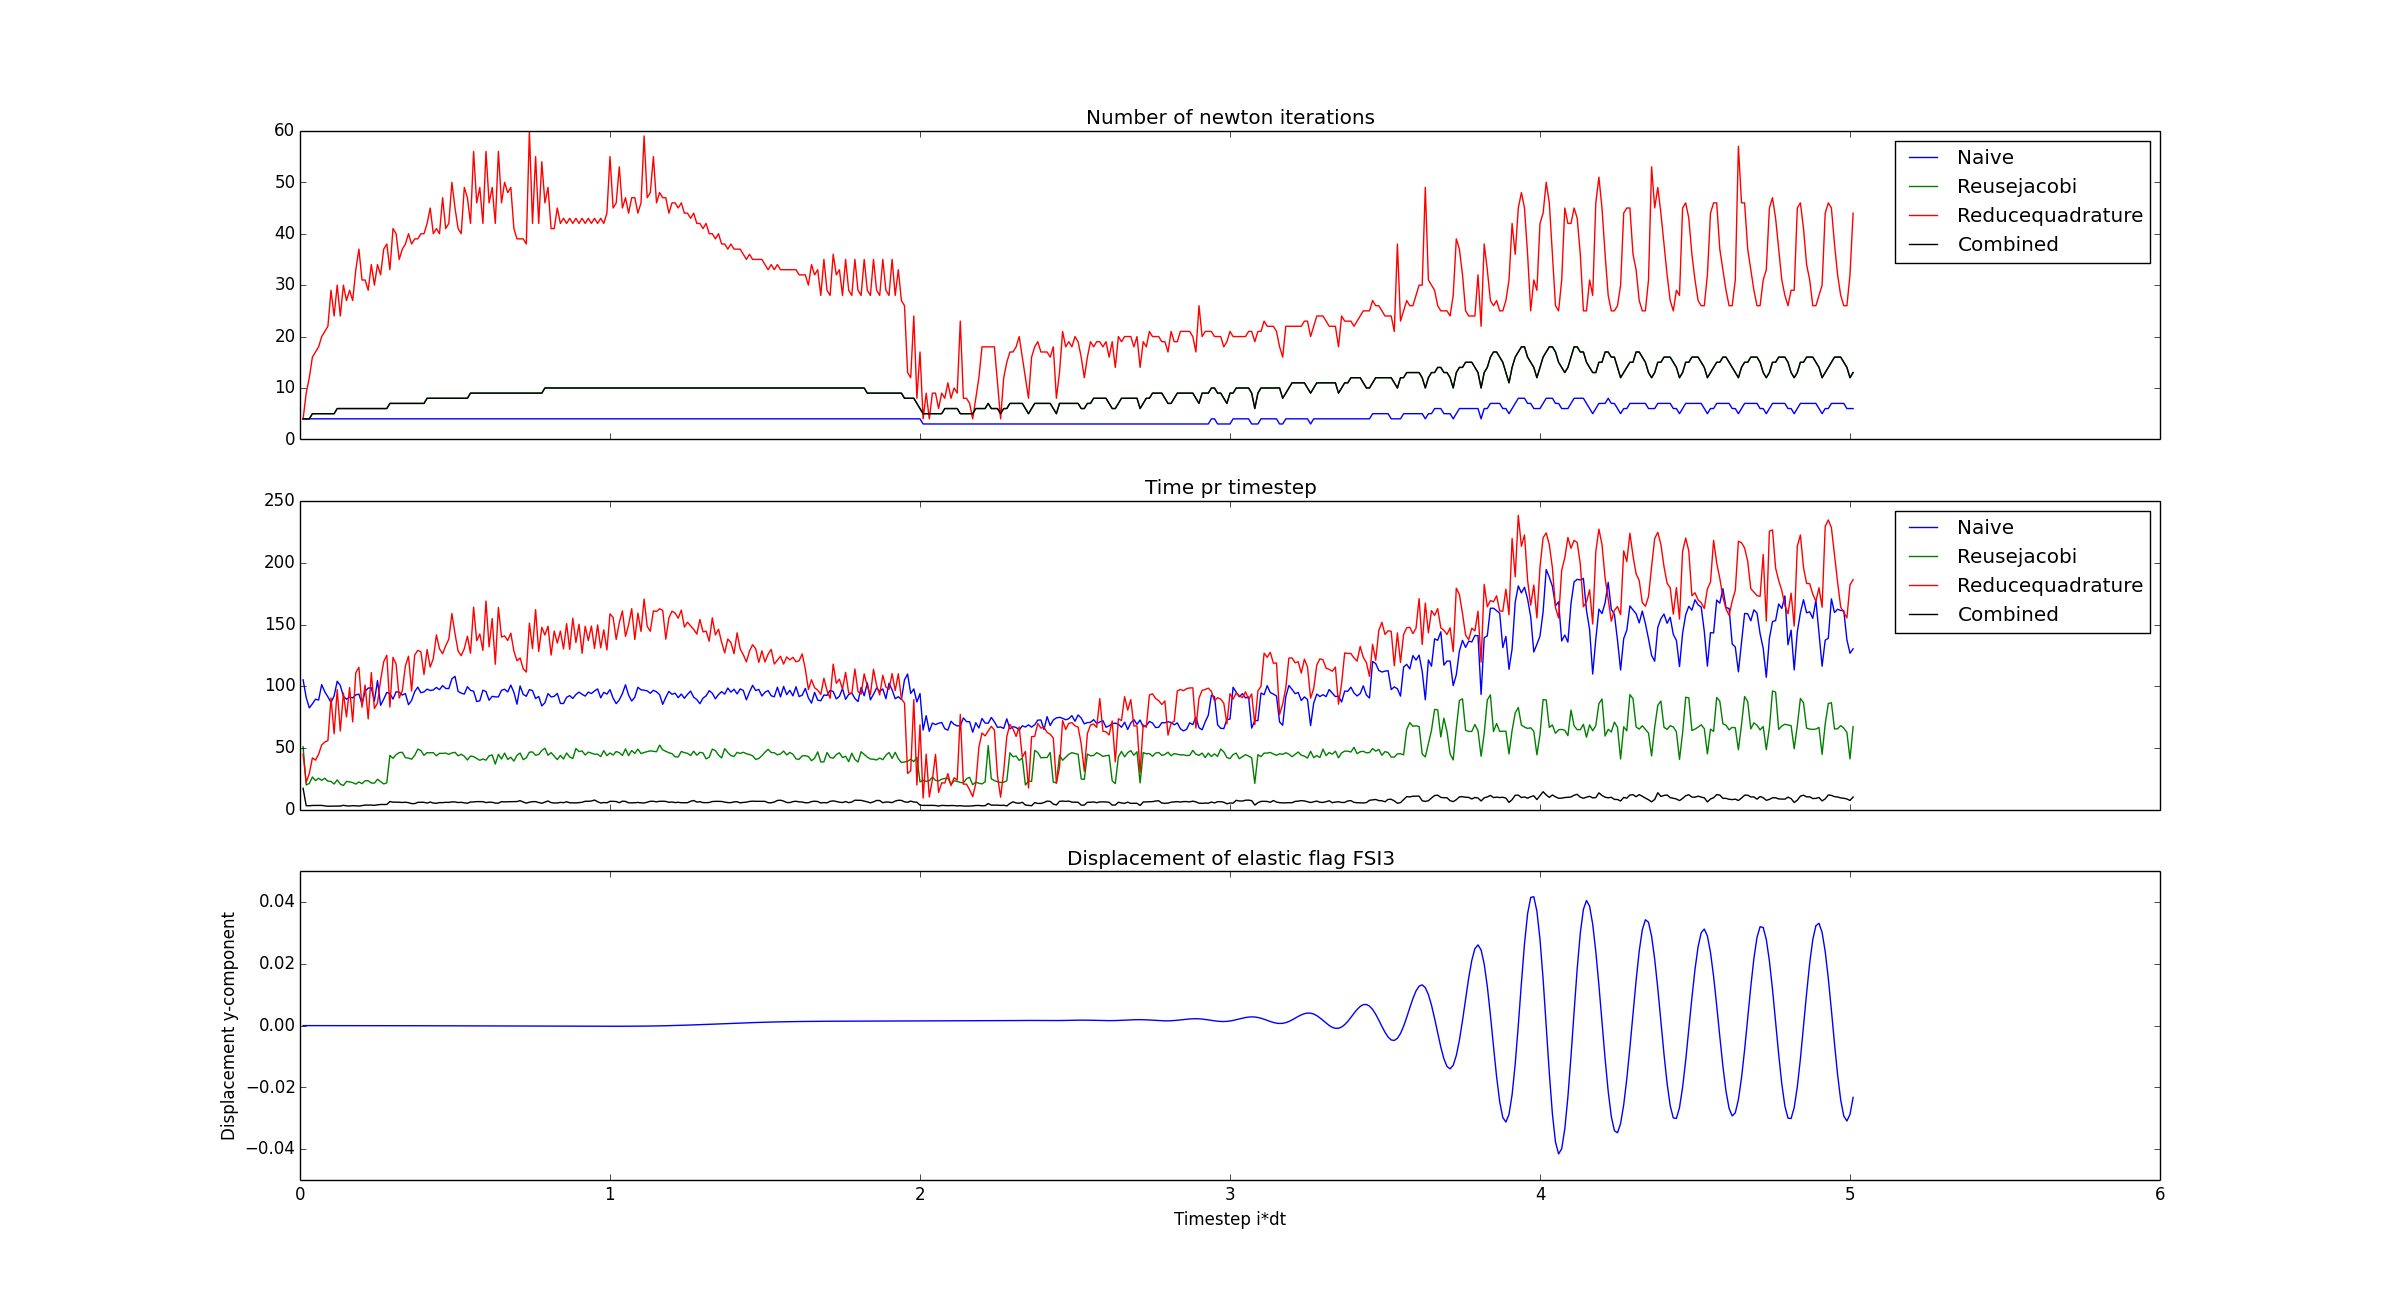
\includegraphics[scale=0.38]{./Fig/itercompare.png}
 \caption{Comparison of speed-up techniques for the laplace mesh model}
 \label{fig:lap_it}
\end{figure}

\begin{figure}[h!]
 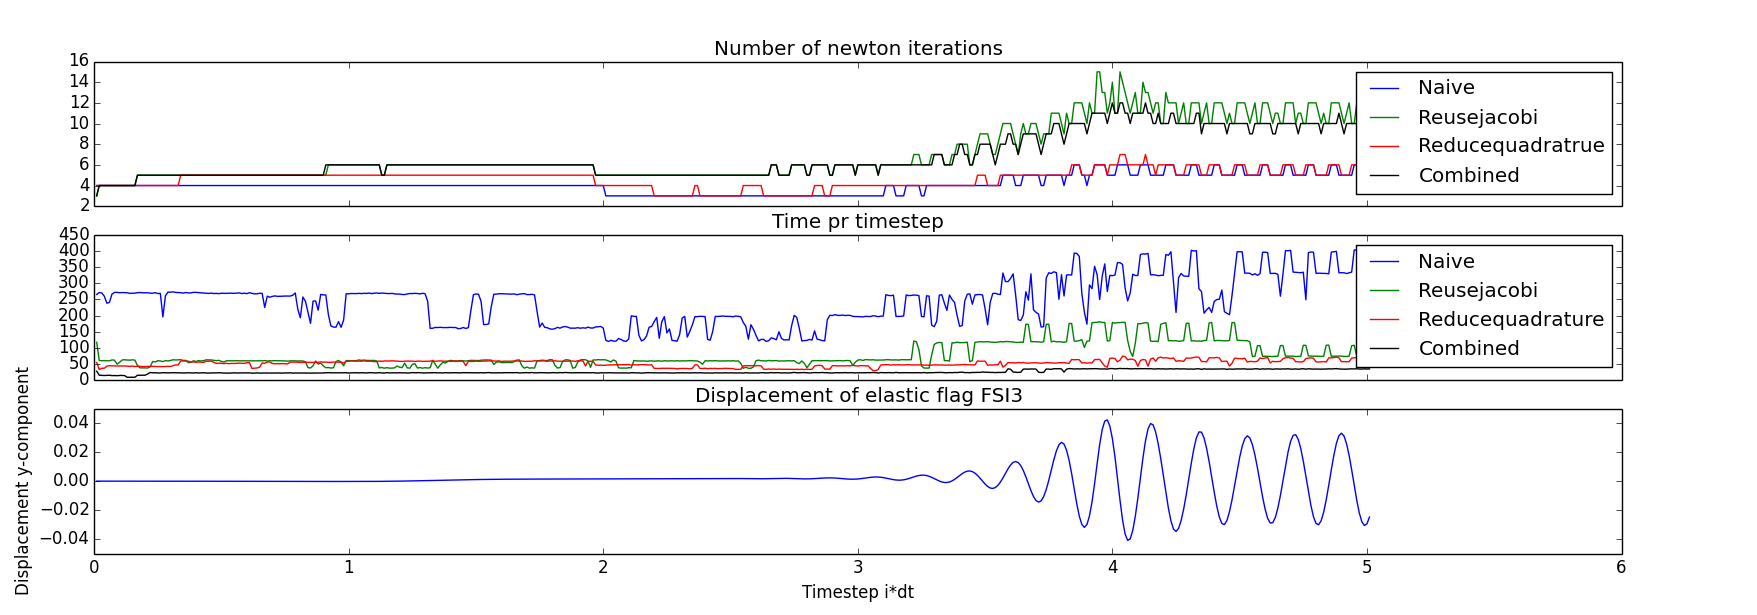
\includegraphics[scale=0.38]{./Fig/bi_compareit.png}
 \caption{Comparison of speed-up techniques for the biharmonic type 1 mesh model}
  \label{fig:bi_it}
\end{figure}


\begin{table}[h!]
\centering
\caption{Comparison of speedup techniques}
\label{my-label}
\begin{tabular}{ |p{2.8cm}|p{2.2cm}|p{2.4cm}|p{2.4cm}|p{2.4cm}|p{2.4cm}| }
 \hline
  \multicolumn{6}{|c|}{Laplace} \\
 \hline
Implementation & Naive&Buffering&Reusejacobi&Reducequadrature&Combined \\
\hline
 Mean time pr timestep &123.10  & 159.85  & 61.31  & 31.43  & 11.11  \\
\hline
Mean iteration &4.50  & 7.79  & 10.22  & 10.08  & 10.22  \\
\hline
Speedup ratio& -  & 0.12  & 0.50  & 0.74  & 0.91  \\
  \hline
  \multicolumn{6}{|c|}{Biharmonic Type 1} \\
 \hline
Implementation & Naive & Buffering & Reusejacobi & Reducequad &Combined \\
\hline
 Mean time pr timestep &243.39  & 307.67  & 76.77  & 51.64  & 24.87  \\
\hline
Mean iteration &4.14  & 6.21  & 7.19  & 4.67  & 6.81  \\
\hline
Speedup ration& -  & -0.26  & 0.68  & 0.79  & 0.90  \\
\hline
\end{tabular}
\end{table}


\newpage
\chapter{Conclusion and further research}

In this thesis, a monolithic fluid-structure interaction solver in an arbitrary Lagrangian Eulerian description have been presented. This inline with the original goal of this thesis. However, verification of code was not achieved, however successful validation through the benchmark presented in~\cite{Hron2006} indicates the code still represents the mathematical model correctly enough. Thus it opens up the possibility that the verification of code test it self might have been erroneous. \\

An investigation of long term temporal stability of the FSI benchmark showed the implicit Crank-Nicolson was not applicable for time steps $\Delta t > 0.001$. To overcome the stability issues, a shifted Crank-Nicolson scheme was introduced, were long time temporal stability was obtained for $\Delta t \leq 0.01$. Software profiling motivated run-time optimizations of the Newton solver, where a combination of Jacobian reuse and lower-order polynomials to assemble the Jacobian matrix proved most beneficial in terms of computational efficiency. \\

In order to further explore all aspects of the FSI problem, I have also compared three different mesh lifting operators, focusing on mesh regularity and computational efficiency. The Laplace lifting operator proved to be the most efficient method, while the biharmonic operator was the most rigorous, however at the cost of computational cost. The linear elastic model failed for all tests expect the FSI-1 problem, meaning it was only valid for small deformations. 

\newpage
\subsection*{Future research}
To pursue a successful verification of code is the primary future goal, which is necessary remove any doubt that the mathematical model is solved correctly. In addition, several extensions are possible. Several publications have showed the linear elastic lifiting operator applicable for a wide range of FSI problems. Therefore, further investigation is planned to investigate why the operator did not perform in my work. \\

Hoping to extend into 3D simulations, an implementation of iterative Krylov methods by block preconditioning are necessary, to overcome the CPU demanding nature of the monolithic FSI formulation. A substantial amount of time during the work of this thesis have been put into trying to implement the partitioned algorithm presented in \cite{Fernandez2007}. In the end, I was not able to finalize this project, but future research will be spent on finding the last mistakes. A projection method would allow for a wider variety of fluid schemes, making the whole fluid equation linear. Thus, having the potential of further speeding up the solution process.

\newpage
\begin{appendices}
\addtocontents{toc}{\protect\setcounter{tocdepth}{0}}

%  \chapter{First appendix}
%  \section{First section}
%  \section{Second section}

  %\chapter{Second appendix}
  %\section{First section}
  %\section{Second section}
%\end{appendices}


\chapter{The deformation gradient}
\ref{appendix:defgrad}
%\section{The deformation gradient}
Deformation is a major property of interest when a continuum is influenced by external and internal forces.  The deformation results in relative change of position of material particles, called \textit{strain}. and is the primary property that causes and describe \textit{stress}. Strain is purely an observation, and it is not dependent on the material of interest. However one expects that a material undergoing strain, will give  forces within a continuum due to neighboring material particles interacting with one another. Therefore one derive material specific models to describe how a certain material will react to a certain amount of strain. These strain measures are used to define models for \textit{stress}, which is responsible for the deformation in materials \cite{Holzapfel2000}. Stress is defined as the internal forces that particles within a continuous material exert on each other, with dimension force per unit area.  \\

The equations of continuum mechanics can be derived with respect to either a deformed or undeformend configuration. The choice of refering our equations to the current or reference configuration is indifferent from a theoretical point of view. In practice however this choice can have a severe impact on our strategy of solution methods and physical of modelling.   \cite{Wriggers2006}. Regardless of configuration, the \textit{deformation gradient} and \textit{determinant of the deformation gradient} are essential measurement in structure mechanics. 
By \cite{Richter2016}, both configurations are considered.

\subsubsection*{Reference configuration}
\begin{defn}
Let $\hat{u}$ be a differential deformation field in the \textit{reference} configuration, $I$ be the Identity matrix and
the gradient $\hat{\nabla} = (\frac{\partial}{\partial x}, \frac{\partial}{\partial y}, \frac{\partial}{\partial z}) $. Then the \textit{deformation gradient} is given by,
\begin{align}
\bat{F} = I + \hat{\nabla} \bat{u} 
\end{align} 
\textit{expressing the local change of relative position under deformation.}
\end{defn}

\begin{defn}
Let $\hat{u}$ be a differential deformation field in the \textit{reference} configuration, $I$ be the Identity matrix and
the gradient $\hat{\nabla} = (\frac{\partial}{\partial x}, \frac{\partial}{\partial y}, \frac{\partial}{\partial z}) $. Then the \textit{determinant of the deformation gradient} is given by,
\begin{align}
J = det(\bat{F}) = det( I + \hat{\nabla} \bat{u} )
\end{align} 
\textit{expressing the local change of volume the configuration.}
\end{defn}

From the assumption of linear operator \textbf{F}, and no two particles $\bat{x}_a, \bat{x}_b \in \ha{V}$ occupy the same location for some time $V(t)$,  J to be greater than 0 \cite{Wriggers2006}. \\ \\

\subsubsection*{Current configuration}
\begin{defn}
Let $\mathbf{u}$ be a differential deformation field in the \textit{reference} configuration, $I$ be the Identity matrix and
the gradient $\mathbf{\nabla} = (\frac{\partial}{\partial x}, \frac{\partial}{\partial y}, \frac{\partial}{\partial z}) $. Then the \textit{deformation gradient} is given by,
\begin{align}
\mathbf{F} = I - \mathbf{\nabla} \mathbf{u} 
\end{align} 
\textit{expressing the local change of relative position under deformation.}
\end{defn}

\begin{defn}
Let $\mathbf{u}$ be a differential deformation field in the \textit{reference} configuration, $I$ be the Identity matrix and
the gradient $\mathbf{\nabla} = (\frac{\partial}{\partial x}, \frac{\partial}{\partial y}, \frac{\partial}{\partial z}) $. Then the \textit{determinant of the deformation gradient} is given by,
\begin{align}
J = det(\mathbf{F}) = det( I - \mathbf{\nabla} \mathbf{u} )
\end{align} 
\textit{expressing the local change of volume the configuration.}
\end{defn}


\chapter{Strain tensor}
\ref{appendix:strainapp}
The equations describing forces on our domain can be derived in accordinance with the current or reference configuration. With this in mind, different measures of strain can be derived with respect to which configuration we are interested in. We will here by \cite{Richter2016} show the most common measures of strain. We will first introduce the right \textit{Cauchy-Green} tensor \textbf{C}, which is one of the most used strain measures \cite{Wriggers2006}. \\ Uttrykk 1.3 fra Godboka, LAG TEGNING \\ 

Let $\ha{x}, \ha{y} \in \ha{V}$ be two points in our referemce configuration and let $\ha{a} = \ha{y} - \ha{x}$ denote the
length of the line bewtween these two points. As our domain undergoes deformation let 
$x = \ha{x} + \hat{u}( \ha{x} ) $ and $x = \ha{y} + \hat{u}( \ha{y} )  $ be the position of our points in the current configuration, and let $a = y - x$ be our new line segment. By \cite{Richter2016} we have by first order Taylor expansion

\begin{align*}
&y - x = \ha{y} + \hat{u}(\ha{y}) - \ha{x} - \hat{u}(\ha{x}) = \
\ha{y} - \ha{x} + \hat{\nabla}\ha{u}(\ha{x}) (\ha{y} - \ha{x}) 
+ \mathcal{O}(|\ha{y} - \ha{x} |^2) \\
&\frac{y - x}{|\ha{y} - \ha{x}|} = [I + \hat{\nabla}\hat{u}(\ha{x} ]  
\frac{\ha{y} - \ha{x}}{|\ha{y} - \ha{x}|} + \mathcal{O}(|\ha{y} - \ha{x} |) 
\end{align*}

This detour from \cite{Richter2016}  we have that 
\begin{align*}
&a = y - x = \hat{F}(\ha{x})\ha{a} +  \mathcal{O}(|\ha{a} |^2) \\
&|a| = \sqrt{ (\hat{F}\ha{a},\hat{F}\ha{a})+ \mathcal{O} (|\ha{a}^3|)  } = 
 \sqrt{ (\ha{a}^T, \hat{F}^T\hat{F}\ha{a})} + \mathcal{O} (|\ha{a}^2|)  
\end{align*}

We let $\ha{C} = \ha{F}^T \ha{F}$ denote the right \textit{Cauchy-Green tensor}.
By observation the Cauchy-Green tensor is not zero at the reference configuration 
\begin{align*}
\ha{C} =  \ha{F}^T \ha{F} = (I + \hat{\nabla} \ha{u})^T (I + \hat{\nabla} \ha{u}) = 1
\end{align*}

Hence it is convenient to introduce a tensor which is zero at the reference configuration. We define the \textit{Grenn-Lagrange strain tensor}, which arises from the squard rate of change of the linesegment \ha{a} and \textit{a}. By using the definition of the Cauchy-Green tensor we have the relation
\begin{align*}
&\frac{1}{2}(|a|^2 + |\ha{a}|^2) = \frac{1}{2}(\ha{a}^T\hat{C}\ha{a}
 -\ha{a}^T \ha{a} ) + \mathcal{O}(|\ha{a}^3| = 
 \ha{a}^T \big(\frac{1}{2} (\hat{F}^T \hat{F} - I) \big) \ha{a} 
 + \mathcal{O}(\ha{a}^3) \\
&\hat{E} = \frac{1}{2}(\hat{C} - I)
\end{align*}

Both the \textit{right Cauchy-Green tensor} $\hat{C}$ and the \textit{Green-Lagrange} $\hat{E}$ are refered to the Lagrangian coordinate system, hence the \textit{reference configuration}. \\
Using similar arguments (see \cite{Richter2016}, compsda) Eulerian counterparts of the Lagrangian stress tensors can be derived.

The \textit{left Cauchy-Green} strain tensor 
\begin{align*}
\mathbf{b} = \ha{F} \ha{F}^T = 
\end{align*}
and the \textit{Euler-Almansi} strain tensor
\begin{align*}
\mathbf{e} = \frac{1}{2} (I - \hat{F}^{-1}\hat{F}^{-T}) = \hat{F}^{-1}\hat{E}\hat{F}^{T}
\end{align*}

\end{appendices}


\bibliographystyle{plain}
\bibliography{./Cite/Books,./Cite/ALECoupled,./Cite/Decoupled,./Cite/NavierStokes,./Cite/Verification,./Cite/EulerianFormulation,./Cite/Meshupdate}
\end{document}  
